\documentclass[11pt,twoside]{article}

\usepackage[table,xcdraw]{xcolor}
\usepackage{float}

\newcommand{\reporttitle}{Introduction to Machine Learning}

\newcommand{\reporttype}{Coursework 1 \\ \vspace{0.5cm} Decision Trees}
\newcommand{\probdef}[1]{\textbf{Problem:}  #1 \\ \\ \textbf{Answer:}}

% include files that load packages and define macros
%%%%%%%%%%%%%%%%%%%%%%%%%%%%%%%%%%%%%%%%%
% University Assignment Title Page 
% LaTeX Template
% Version 1.0 (27/12/12)
%
% This template has been downloaded from:
% http://www.LaTeXTemplates.com
%
% Original author:
% WikiBooks (http://en.wikibooks.org/wiki/LaTeX/Title_Creation)
%
% License:
% CC BY-NC-SA 3.0 (http://creativecommons.org/licenses/by-nc-sa/3.0/)
% 
% Instructions for using this template:
% This title page is capable of being compiled as is. This is not useful for 
% including it in another document. To do this, you have two options: 
%
% 1) Copy/paste everything between \begin{document} and \end{document} 
% starting at \begin{titlepage} and paste this into another LaTeX file where you 
% want your title page.
% OR
% 2) Remove everything outside the \begin{titlepage} and \end{titlepage} and 
% move this file to the same directory as the LaTeX file you wish to add it to. 
% Then add \input{./title_page_1.tex} to your LaTeX file where you want your
% title page.
%
%----------------------------------------------------------------------------------------
%	PACKAGES AND OTHER DOCUMENT CONFIGURATIONS
%----------------------------------------------------------------------------------------
\usepackage{ifxetex}
\usepackage{textpos}
\usepackage{natbib}
\usepackage{kpfonts}
\usepackage[a4paper,hmargin=2.8cm,vmargin=2.0cm,includeheadfoot]{geometry}
\usepackage{ifxetex}
\usepackage{stackengine}
\usepackage{tabularx,longtable,multirow,subfigure,caption}%hangcaption
\usepackage{fncylab} %formatting of labels
\usepackage{fancyhdr}
\usepackage{color}
\usepackage[tight,ugly]{units}
\usepackage{url}
\usepackage{float}
\usepackage[english]{babel}
\usepackage{amsmath}
\usepackage{graphicx}
\usepackage[colorinlistoftodos]{todonotes}
\usepackage{dsfont}
\usepackage{epstopdf} % automatically replace .eps with .pdf in graphics
\usepackage{natbib}
\usepackage{backref}
\usepackage{array}
\usepackage{latexsym}
\usepackage{etoolbox}

\usepackage{enumerate} % for numbering with [a)] format 



\ifxetex
\usepackage{fontspec}
\setmainfont[Scale=.8]{OpenDyslexic-Regular}
\else
\usepackage[pdftex,pagebackref,hypertexnames=false,colorlinks]{hyperref} % provide links in pdf
\hypersetup{pdftitle={},
  pdfsubject={}, 
  pdfauthor={\reportauthor},
  pdfkeywords={}, 
  pdfstartview=FitH,
  pdfpagemode={UseOutlines},% None, FullScreen, UseOutlines
  bookmarksnumbered=true, bookmarksopen=true, colorlinks,
    citecolor=black,%
    filecolor=black,%
    linkcolor=black,%
    urlcolor=black}
\usepackage[all]{hypcap}
\fi

\usepackage{tcolorbox}

% various theorems
\usepackage{ntheorem}
\theoremstyle{break}
\newtheorem{lemma}{Lemma}
\newtheorem{theorem}{Theorem}
\newtheorem{remark}{Remark}
\newtheorem{definition}{Definition}
\newtheorem{proof}{Proof}

% example-environment
\newenvironment{example}[1][]
{ 
\vspace{4mm}
\noindent\makebox[\linewidth]{\rule{\hsize}{1.5pt}}
\textbf{Example #1}\\
}
{ 
\noindent\newline\makebox[\linewidth]{\rule{\hsize}{1.0pt}}
}



%\renewcommand{\rmdefault}{pplx} % Palatino
% \renewcommand{\rmdefault}{put} % Utopia

\ifxetex
\else
\renewcommand*{\rmdefault}{bch} % Charter
\renewcommand*{\ttdefault}{cmtt} % Computer Modern Typewriter
%\renewcommand*{\rmdefault}{phv} % Helvetica
%\renewcommand*{\rmdefault}{iwona} % Avant Garde
\fi

\setlength{\parindent}{0em}  % indentation of paragraph

\setlength{\headheight}{14.5pt}
\pagestyle{fancy}
\fancyfoot[ER,OL]{\thepage}%Page no. in the left on
                                %odd pages and on right on even pages
\fancyfoot[OC,EC]{\sffamily }
\renewcommand{\headrulewidth}{0.1pt}
\renewcommand{\footrulewidth}{0.1pt}
\captionsetup{margin=10pt,font=small,labelfont=bf}


%--- chapter heading

\def\@makechapterhead#1{%
  \vspace*{10\p@}%
  {\parindent \z@ \raggedright %\sffamily
        %{\Large \MakeUppercase{\@chapapp} \space \thechapter}
        %\\
        %\hrulefill
        %\par\nobreak
        %\vskip 10\p@
    \interlinepenalty\@M
    \Huge \bfseries 
    \thechapter \space\space #1\par\nobreak
    \vskip 30\p@
  }}

%---chapter heading for \chapter*  
\def\@makeschapterhead#1{%
  \vspace*{10\p@}%
  {\parindent \z@ \raggedright
    \sffamily
    \interlinepenalty\@M
    \Huge \bfseries  
    #1\par\nobreak
    \vskip 30\p@
  }}
  



% %%%%%%%%%%%%% boxit
\def\Beginboxit
   {\par
    \vbox\bgroup
	   \hrule
	   \hbox\bgroup
		  \vrule \kern1.2pt %
		  \vbox\bgroup\kern1.2pt
   }

\def\Endboxit{%
			      \kern1.2pt
		       \egroup
		  \kern1.2pt\vrule
		\egroup
	   \hrule
	 \egroup
   }	

\newenvironment{boxit}{\Beginboxit}{\Endboxit}
\newenvironment{boxit*}{\Beginboxit\hbox to\hsize{}}{\Endboxit}



\allowdisplaybreaks

\makeatletter
\newcounter{elimination@steps}
\newcolumntype{R}[1]{>{\raggedleft\arraybackslash$}p{#1}<{$}}
\def\elimination@num@rights{}
\def\elimination@num@variables{}
\def\elimination@col@width{}
\newenvironment{elimination}[4][0]
{
    \setcounter{elimination@steps}{0}
    \def\elimination@num@rights{#1}
    \def\elimination@num@variables{#2}
    \def\elimination@col@width{#3}
    \renewcommand{\arraystretch}{#4}
    \start@align\@ne\st@rredtrue\m@ne
}
{
    \endalign
    \ignorespacesafterend
}
\newcommand{\eliminationstep}[2]
{
    \ifnum\value{elimination@steps}>0\leadsto\quad\fi
    \left[
        \ifnum\elimination@num@rights>0
            \begin{array}
            {@{}*{\elimination@num@variables}{R{\elimination@col@width}}
            |@{}*{\elimination@num@rights}{R{\elimination@col@width}}}
        \else
            \begin{array}
            {@{}*{\elimination@num@variables}{R{\elimination@col@width}}}
        \fi
            #1
        \end{array}
    \right]
    & 
    \begin{array}{l}
        #2
    \end{array}
    &%                                    moved second & here
    \addtocounter{elimination@steps}{1}
}
\makeatother

%% Fast macro for column vectors
\makeatletter  
\def\colvec#1{\expandafter\colvec@i#1,,,,,,,,,\@nil}
\def\colvec@i#1,#2,#3,#4,#5,#6,#7,#8,#9\@nil{% 
  \ifx$#2$ \begin{bmatrix}#1\end{bmatrix} \else
    \ifx$#3$ \begin{bmatrix}#1\\#2\end{bmatrix} \else
      \ifx$#4$ \begin{bmatrix}#1\\#2\\#3\end{bmatrix}\else
        \ifx$#5$ \begin{bmatrix}#1\\#2\\#3\\#4\end{bmatrix}\else
          \ifx$#6$ \begin{bmatrix}#1\\#2\\#3\\#4\\#5\end{bmatrix}\else
            \ifx$#7$ \begin{bmatrix}#1\\#2\\#3\\#4\\#5\\#6\end{bmatrix}\else
              \ifx$#8$ \begin{bmatrix}#1\\#2\\#3\\#4\\#5\\#6\\#7\end{bmatrix}\else
                 \PackageError{Column Vector}{The vector you tried to write is too big, use bmatrix instead}{Try using the bmatrix environment}
              \fi
            \fi
          \fi
        \fi
      \fi
    \fi
  \fi 
}  
\makeatother

\robustify{\colvec}

%%% Local Variables: 
%%% mode: latex
%%% TeX-master: "notes"
%%% End: 
 % various packages needed for maths etc.
% quick way of adding a figure
\newcommand{\fig}[3]{
 \begin{center}
 \scalebox{#3}{\includegraphics[#2]{#1}}
 \end{center}
}

%\newcommand*{\point}[1]{\vec{\mkern0mu#1}}
\newcommand{\ci}[0]{\perp\!\!\!\!\!\perp} % conditional independence
\newcommand{\point}[1]{{#1}} % points 
\renewcommand{\vec}[1]{{\boldsymbol{{#1}}}} % vector
\newcommand{\mat}[1]{{\boldsymbol{{#1}}}} % matrix
\newcommand{\R}[0]{\mathds{R}} % real numbers
\newcommand{\Z}[0]{\mathds{Z}} % integers
\newcommand{\N}[0]{\mathds{N}} % natural numbers
\newcommand{\nat}[0]{\mathds{N}} % natural numbers
\newcommand{\Q}[0]{\mathds{Q}} % rational numbers
\ifxetex
\newcommand{\C}[0]{\mathds{C}} % complex numbers
\else
\newcommand{\C}[0]{\mathds{C}} % complex numbers
\fi
\newcommand{\tr}[0]{\text{tr}} % trace
\renewcommand{\d}[0]{\mathrm{d}} % total derivative
\newcommand{\inv}{^{-1}} % inverse
\newcommand{\id}{\mathrm{id}} % identity mapping
\renewcommand{\dim}{\mathrm{dim}} % dimension
\newcommand{\rank}[0]{\mathrm{rk}} % rank
\newcommand{\determ}[1]{\mathrm{det}(#1)} % determinant
\newcommand{\scp}[2]{\langle #1 , #2 \rangle}
\newcommand{\kernel}[0]{\mathrm{ker}} % kernel/nullspace
\newcommand{\img}[0]{\mathrm{Im}} % image
\newcommand{\idx}[1]{{(#1)}}
\DeclareMathOperator*{\diag}{diag}
\newcommand{\E}{\mathds{E}} % expectation
\newcommand{\var}{\mathds{V}} % variance
\newcommand{\gauss}[2]{\mathcal{N}\big(#1,\,#2\big)} % gaussian distribution N(.,.)
\newcommand{\gaussx}[3]{\mathcal{N}\big(#1\,|\,#2,\,#3\big)} % gaussian distribution N(.|.,.)
\newcommand{\gaussBig}[2]{\mathcal{N}\left(#1,\,#2\right)} % see above, but with brackets that adjust to the height of the arguments
\newcommand{\gaussxBig}[3]{\mathcal{N}\left(#1\,|\,#2,\,#3\right)} % see above, but with brackets that adjust to the height of the arguments
\DeclareMathOperator{\cov}{Cov} % covariance (matrix) 
\ifxetex
\renewcommand{\T}[0]{^\top} % transpose
\else
\newcommand{\T}[0]{^\top}
\fi
% matrix determinant
\newcommand{\matdet}[1]{
\left|
\begin{matrix}
#1
\end{matrix}
\right|
}



%%% various color definitions
\definecolor{darkgreen}{rgb}{0,0.6,0}

\newcommand{\blue}[1]{{\color{blue}#1}}
\newcommand{\red}[1]{{\color{red}#1}}
\newcommand{\green}[1]{{\color{darkgreen}#1}}
\newcommand{\orange}[1]{{\color{orange}#1}}
\newcommand{\magenta}[1]{{\color{magenta}#1}}
\newcommand{\cyan}[1]{{\color{cyan}#1}}


% redefine emph
\renewcommand{\emph}[1]{\blue{\bf{#1}}}

% place a colored box around a character
\gdef\colchar#1#2{%
  \tikz[baseline]{%
  \node[anchor=base,inner sep=2pt,outer sep=0pt,fill = #2!20] {#1};
    }%
}%
 % short-hand notation and macros

%%%%%%%%%%%%%%%%%%%%%%%%%%%%
\setlength{\parindent}{1cm} % Default is 15pt.

\begin{document}
% front page
% Last modification: 2016-09-29 (Marc Deisenroth)
\begin{titlepage}

\newcommand{\HRule}{\rule{\linewidth}{0.5mm}} % Defines a new command for the horizontal lines, change thickness here


%----------------------------------------------------------------------------------------
%	LOGO SECTION
%----------------------------------------------------------------------------------------


\includegraphics[width = 4cm]{./figures/imperial}\\[0.5cm] 

\begin{center} % Center remainder of the page

%----------------------------------------------------------------------------------------
%	HEADING SECTIONS
%----------------------------------------------------------------------------------------
\textsc{\LARGE \reporttype}\\[1.5cm] 
\textsc{\Large Imperial College London}\\[0.5cm] 
\textsc{\large Department of Computing}\\[0.5cm] 
%----------------------------------------------------------------------------------------
%	TITLE SECTION
%----------------------------------------------------------------------------------------

\HRule \\[0.4cm]
{ \huge \bfseries \reporttitle}\\ % Title of your document
\HRule \\[1.5cm]
\end{center}
%----------------------------------------------------------------------------------------
%	AUTHOR SECTION
%----------------------------------------------------------------------------------------

%\begin{minipage}{0.4\hsize}
\begin{flushleft} \large
\textit{Author:}\\
\reportauthor~(CID: \cid) \\% Your name 
\textit{Email:} \\
\reportemail
\end{flushleft}
\vspace{2cm}
\makeatletter
Date: \@date 

\vfill % Fill the rest of the page with whitespace



\makeatother


\end{titlepage}



\thispagestyle{empty}
\renewcommand{\contentsname}{Table of Contents}
\setcounter{tocdepth}{2}
{\hypersetup{linkcolor=black} % Locally black links so they don't stand out here
\tableofcontents
% \addtocontents{toc}{\par\nobreak \mbox{}\hfill{\bf Page}\par\nobreak}
% \newpage
%

% \addtocontents{lot}{\par\nobreak\textbf{{\scshape Table} \hfill Page}\par\nobreak}
%
\listoffigures
% \addtocontents{lof}{\par\nobreak\textbf{{\scshape Figure} \hfill Page}\par\nobreak}
\listoftables

}
\newpage
%%%%%%%%%%%%%%%%%%%%%%%%%%%% Main document

\setcounter{page}{1}
\section{Introduction}
We report on the efficacy of a decision tree created to predict which of four rooms an individual is in based on the strength of seven WiFi signal readings. To gain an accurate measure of model performance, we implemented 10-fold cross validation and averaged our results to gain global classification accuracy, precision, recall and F1 score. Trees were also pruned to mitigate effects of overfitting, and were trained using both a clean and noisy dataset. Our results show that trees trained on the clean dataset perform with greater accuracy and gain little from the pruning procedure. Inversely, trees trained on the noisy dataset perform considerably worse, but experience a significant increase in performance after pruning. 

Figures of trees before and after pruning as well as tables of results are provided in \autoref{app:tree_figure} \& \autoref{app:results} respectively.

\section{Implementation}
\subsection{Decision Tree Learning}
Our decision tree algorithm is a recursive function which stores data as a nested dictionary. Our algorithm closely follows that in Algorithm 1 in the coursework specification so we will not repeat it here for the sake of brevity. The entropy quantifies the total amount of uncertainty in the system, therefore we implement a  find\_split function which determines the feature and value to split on based on maximising the entropy gain (hence it is a greedy algorithm); this operates as follows:

\begin{algorithm}
\footnotesize
\SetAlgoLined
\KwResult{Get feature \& value for splitting to deliver max entropy gain}
 \For{feature in Features}{
  sort data by feature\;
  \For{unique value in feature}{
   Split data into $subset_A, subset_B$ using this value\;
    \For{$subset_A, subset_B$}{
    Compute entropy for sub dataset (using \autoref{eq:entropy})\;
    }
   Compute entropy gain from splitting on feature (using \autoref{eq:entropy_gain})\;
   Return value \& entropy gain for max entropy gain\;}
  Return feature \& value for max entropy gain from splitting on each feature\;
 }
\caption{Determining splitting feature and feature value}\label{alg:splitting}
\end{algorithm}
\noindent
Where the quantities allowing us to gauge the information contained within a set of labels are the entropy, $H$, and gain, defined respectively as: 
\begin{align}
    \begin{split}
        H(data)= \sum_{l=0}^{L} \tfrac{|data \: with \: label \: l|}{|data|}  \operatorname{log_2}\tfrac{|data \: with \: label \: l|}{|data|} \quad \textnormal{and}
    \label{eq:entropy}
    \end{split} \\
    \begin{split}
            Gain = H(dataset) - \begin{pmatrix} \frac{|subset_A|} {|dataset|}H(subset_A)+\frac{|subset_B|}{|dataset|}H(subset_B) \end{pmatrix}.
    \label{eq:entropy_gain}
    \end{split}
\end{align}
\noindent
Our decision\_tree\_learning function therefore constructs the tree by calling find\_split initially on the whole dataset, then splitting on the feature and value returned, and recursively repeating this process until exhaustion. When the sub dataset from a split contains only a single label, then a leaf node is returned (with this label), otherwise a dictionary is returned and the recursion continues.

\subsection{K-fold Cross Validation}

Our evaluation was performed using 10-fold cross validation in order to determine a robust measure of our algorithm's performance; accounting for the potential of overfitting to yield deceptively high accuracies, and for statistical fluctuations originating from shuffling the data to result in easier test sets. \textcolor{red!50!black}{Algorithm}~\ref{alg:crossvalidation} details our implementation of k-fold cross validation:

\begin{algorithm}
\footnotesize
\SetAlgoLined
\KwResult{Confusion matrices for K best pruned trees}
Shuffle data\;
Split data into K folds, each with (data\_length / K) rows\;
confusion\_matrices = []\;
 \For{test\_fold in folds}{
  test\_data = test\_fold\;
  folds\_inner = folds except test\_fold\;
  confusion\_matrices\_inner = []\;
  \For{val\_fold in folds\_inner}{
    data\_validation = fold\_inner\;
    data\_train = folds\_inner except val\_fold\;
    tree $\leftarrow$ create tree on training data\;
    pruned\_tree $\leftarrow$ prune tree using validation data\;
    confusion\_matrix $\leftarrow$ evaluate pruned\_tree using test\_data\;
    Append confusion\_matrix to confusion\_matrices\_inner
    }
  Append the confusion matrix for the tree with the highest classification accuracy in Confusion\_matrices\_inner to Confusion\_matrices\;
  }
\caption{K-fold cross validation} \label{alg:crossvalidation}
\end{algorithm}
\noindent
As shown, our 10 fold cross validation implementation trains 9 trees on an inner loop, prunes each of these using the validation data and tests their performance against test data, saving the best performing tree. This process is then repeated 10 times, once for each outer loop. The result is a list of 10 confusion matrices  representing the best-performing tree from its inner loop. We are careful to ensure that the data is split into 10 folds at the beginning of cross validation and remains that way, ensuring that there is never any overlap between train, test and validation sets. The details as to how these matrices were averaged to compute the global average for our algorithm are discussed in \autoref{sec:average}.

\subsection{Computing Average Results}
\label{sec:average}
To derive meaningful conclusions from the results of running 10-fold cross validation, we average over the metrics calculated for each tested tree in every fold. However, in order to account for potential bias due to imbalances in the features for a given test set, we normalized the confusion matrix by row, i.e., by feature. This procedure resulted in the calculation of a single unbiased confusion matrix for the entire cross validation procedure, from which the recall, precision and F1 were then derived, as discussed in \autoref{sec:evaluation}.
% Now that we have performed cross validation, we would like to report on the accuracy of our model. Given that we have 10 confusion matrices from cross-validation (see above), we must average the results of these in order to report global average results. Note that we do not specify that each of the 10 folds must be equally represented for each class during cross validation, account for the possibility of imbalanced test/validation sets when averaging results. To this end, each matrix was normalised by dividing each row by the total number of examples per class. This step mitigates the risk of introducing bias in favour of the majority class to the evaluation metrics, including accuracy, precision and F1. Once normalised, the mean values were computed for each element across the 10 matrices to produce a global confusion matrix representative of the results of the 10-fold cross validation. From the average confusion matrix, we compute the average recall, precision rates and F1 measure for each class, which discuss further in Section 3. 




\section{Evaluation}
\label{sec:evaluation}
\subsection{Metrics}
The classification accuracy alone provides only a crude measure of model performance. As such, we introduce other useful metrics which can be calculated from the confusion matrix. 
%To this end, we introduce the notation \textbf{TP} (true positive) to refer to the number of samples correctly labelled as True in a dataset, \textbf{FN} (false negative) to refer to the number of samples incorrectly labelled as false, etc.
\noindent
Recall is defined as 
\begin{equation}
\textnormal{Recall}=\frac{\textnormal{True Positive}}{\textnormal{True Positive}+\textnormal{False Negative}},
\end{equation}
capturing how well our model labels the readings from a room compared to the true number of readings from that room.

Precision is defined as
\begin{equation}
\textnormal{Precision}=\frac{\textnormal{True Positive}}{\textnormal{True Positive}+\textnormal{False Positive}},
\end{equation}
and provides a measure of how likely it is that a reading was actually from a given room after the model predicted it was from that room.

The F1 measure is defined as the harmonic mean of precision and recall, taking the form
\begin{equation}
F_{1}=2\cdot\frac{\textnormal{Precision}\cdot \textnormal{Recall}}{\textnormal{Precision}+\textnormal{Recall}}.
\end{equation}
F1 acts as a single metric for performance of the model, combining the precision and recall metrics, taking into account any possible precision-recall trade-off.
% Intuitively, this may be thought of as measuring BLA.\textcolor{red}{Suggestion: }.% It's not necessarily measuring something but a single metric combining the precision and recall metrics, through taking a harmonic mean to take into account any possible precision-recall trade-off



\subsection{Results}
For the clean dataset, before pruning, the average classification rate was 97.1\%, with precision of 99.1\% and 98.6\% for rooms 1 and 4 respectively. The trained trees had relatively more difficulty classifying rooms 2 and 3, however, misclassifying between them to similar degrees (with precision rates of 95.9\% and 94.9\% respectively, and with similar recall rates). The trained decision trees were still generally a good representation of the test set. The full results are shown on \autoref{tab:confusion_clean_unpruned} and \autoref{tab:RPF_unpruned_clean}.

\autoref{tab:rates} shows the classification accuracies which resulted from the cross-validation procedure for both datasets, with and without pruning. We see that for the noisy dataset the average classification rate was 80.1\% before pruning, significantly lower than for the clean dataset. This was predominantly due to additional random noise in the dataset, especially with the recall rates for each class falling to similar levels (around 80\%). In addition, significant misclassification was no longer exclusive to rooms 2 and 3, but spread more evenly amongst all classes. The full results for the noisy dataset are shown on \autoref{tab:confusion_noisy_unpruned} and \autoref{tab:RPF_unpruned_noisy}. Interestingly, pruning increases the classification rate to 88\% for the noisy dataset; see \autoref{sec:pruning_question} for a full discussion (complete results seen in  \autoref{tab:confusion_noisy_pruned} and \autoref{tab:RPF_pruned_noisy}). 

\begin{table}[h!]
\small\addtolength{\tabcolsep}{-5pt}
\centering
\begin{tabular}{|
>{\columncolor[HTML]{EFEFEF}}l |l|l|}
\hline
               & \cellcolor[HTML]{EFEFEF}\textbf{Unpruned} & \cellcolor[HTML]{EFEFEF}\textbf{Pruned} \\ \hline
\textbf{Clean} & 0.971                                     & 0.969                                  \\ \hline
\textbf{Noisy} & 0.801                                     & 0.880                                   \\ \hline
\end{tabular}
\caption[Classification Rates for Datasets Before and After Pruning]{Classification rates for datasets before and after pruning}
\label{tab:rates}
\end{table}
% -- Add average classification rate 1- classification error

% Clean Unpruned rate = 0.971\\
% Clean Pruned rate =  0.0969\\
% Noisy Unpruned rate = 0.801\\
% Noisy Pruned rate = 0.880}
% [FYI we have this in table 9]

\section{Questions}

\subsection{Noisy-Clean Datasets Question}
% \probdef{Is there any difference in the performance
% when using the clean and noisy datasets? If yes/no explain why. Discuss the differences in the overall performance and per class.}
\label{sec:datasets_question}
As highlighted in the previous section, there is an observable difference in the performance when using the clean and noisy datasets (see \autoref{fig:pruning_effect_overview}). The difference in performance can be partly explained from observing how the two datasets differ, as despite having similar mean values for each attribute per class, the variances for attribute-label pairings were greater for the noisy dataset; in particular, the distributions were observed to have tails which were barely present in the clean dataset. Additionally, the decision trees trained on the noisy dataset were both more dense (more nodes) and deeper on average (so long as the depth parameter was unconstrained), resulting from overfitting to noise in the noisy dataset, and thus detrimenting the tree's performance (see \autoref{sec:pruning_question} for elaboration). 

% As a result, when using the noisy dataset, the unconstrained, unpruned decisions trees would look to fit to the noise, particularly lower down in the tree, and hence become more susceptible to overfitting. As seen in Section 3, this results in the markedly lower average classification rate when using the noisy dataset, with the average classification rate falling to c.80\%. The additional random noise can also be observed from the misclassification being no longer isolated between rooms 2 and 3, as with the clean dataset (\autoref{tab:confusion_clean_unpruned}), but spread more evenly amongst all classes (\autoref{tab:confusion_noisy_unpruned}). 

As per \autoref{tab:rates}, whilst pruning improves the performance significantly when using the noisy dataset, increasing the average classification rate to 88.0\%, the noise still prevents the trees from replicating the performance achieved on the clean dataset. This behaviour results from the instability of na\"ive decision trees as a learning algorithm, particularly their susceptibility to overfitting. This instability is evidenced by the fact that the relatively subtle differences between the clean and noisy datasets results in drastically different trees, even in spite of pruning. Note that it is possible to overcome the limitations caused by overfitting more reliably by using the random forest algorithm, whereby one trains an ensemble of uncorrelated trees and takes the most common class output (the mode) as the prediction of the ensemble.
 

\subsection{Pruning Question}
\label{sec:pruning_question}

Our implementation of pruning is recursive and in-place\footnote{%
We refer here to post-pruning, as opposed to pre-pruning in which the emphasis is on restricting parameters such as the maximum depth or number of nodes of the tree, before training}.
\autoref{fig:pruning_algorithm} shows how one step of the recursive algorithm takes place. In essence, the algorithm steps upwards from the bottom left of the tree through to the bottom right, attempting to replace nodes which have two leaf nodes as their children (referred to as \textit{base parents}) for increased classification accuracy. This bottom up recursion is crucial, as it ensures that multiple base parents in a branch can be efficiently replaced with leaf nodes, if deemed beneficial. It is worth noting that the decision to prune based on classification accuracy stems from the nature of the problem which we are attempting to solve. Specifically, as the problem we are solving is the localization of an individual in their home, we are more interested in the average accuracy over long periods of time, especially given that in practice the sampling rate of the wifi signal strenghts would high, and reasonable interpolation would allow us to perform the task of tracking the individual. This would of course not be the approach utilized in a setting such as medical diagnosis, where we specifically aim to minimize the number of false negatives, as flagging something erroneously may be less dertimental than overlooking it\footnote{Especially as most current AI based medical systems would refer your results to a doctor for further inspection.}.
\begin{figure}[H]
    \centering
    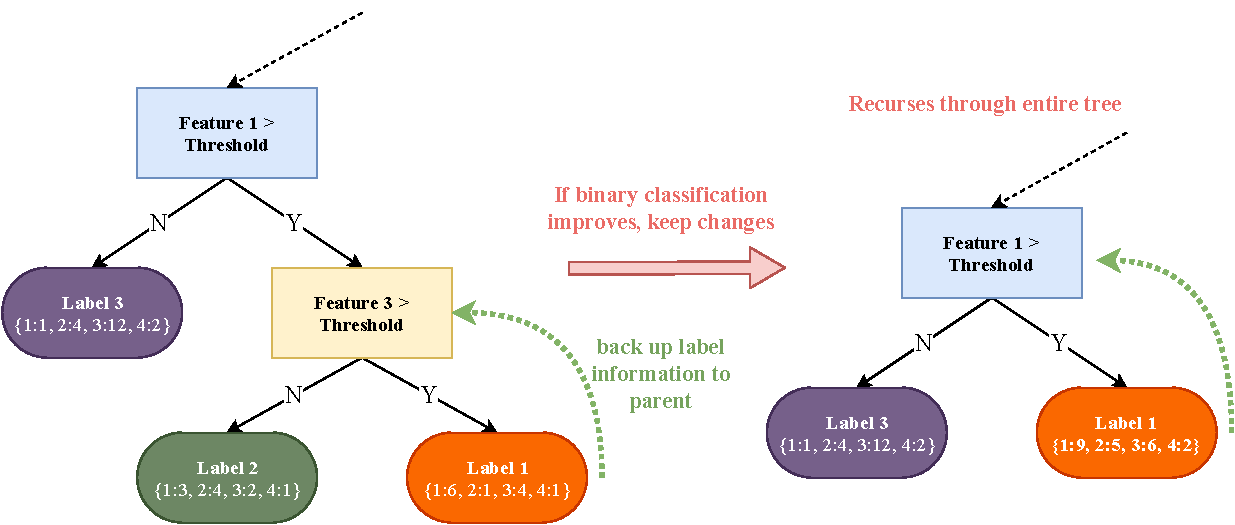
\includegraphics[width=0.8\textwidth]{figures/pruning.pdf}
    \caption[Illustration of Recursive Pruning Algorithm]{A pictorial depiction of a single step in the recursive pruning algorithm, where pruning the node which splits about "Feature 3" improved the classification accuracy, and thus the recursion continued upward. The leaves contain a record of the frequency of labels which were present in their split after training; this is merged after a successful pruning step, and allows the labelling of the resulting leaf node.}
    \label{fig:pruning_algorithm}
\end{figure}
It is worth noting that this pruning algorithm is only guaranteed to find the optimal tree (for a given evaluation set) because decision trees are deterministic, and as splits on one side of the tree are not coupled to those on another. Indeed, if this were not the case, one would have a combinatorial blow up as every base node replacement would have to be evaluated in the context of all other possible base node replacements\footnote{An issue which one faces in highly non-linear optimization problems.}.

Figures~\ref{fig:pruning_example_clean_unpruned} \& \ref{fig:pruning_example_clean_pruned} show examples of pruned and unpruned trees for the case of the clean data set, respectively. Similarly, Figures~\ref{fig:pruning_example_noisy_unpruned} \& \ref{fig:pruning_example_noisy_pruned} show non-pruned and pruned trees for the noisy data set. The latter pair of trees is considerably more interesting as it clearly shows that the effect of pruning is considerably more dramatic for the noisy dataset, owing to the large prevalence of splitting nodes which resulted from overfitting to noise. This effect is illustrated very clearly in  Figure~\ref{fig:nodes}, which shows that the trees overfit significantly to noise, resulting in greater depth and correspondingly more nodes. Consequently, we see that pruning is dramatically beneficial in the case of the noisy dataset, leading to a $\sim8\%$ increase in classification accuracy on average, and dramatically reducing the number of nodes in a typical tree.  

It is also worth noting that whilst \autoref{tab:rates} suggests that pruning worsens the accuracy of the trees trained on the clean dataset. The standard deviation in these results is of order $\sim1\%$, such that little can be confidently read into such deviations.
%However, one could in principle imagine a scenario in which the evaluation set disproportionately features one set of labels, and that these were therefore less present in the training. Under such circumstances, pruning may turn out to be beneficial  STATISTICAL, POTENTIAL MECHANISM VIA DESTRUCTION OF VALID SPLITS UNLIKELY UNLESS UNREPRESENTATIVE EVALUATION DATA.



As shown by these figures, the effect of pruning is to improve the generalizability of our tree by removing splits that were the result of training to noise; instead focusing on the broader, but more reliable, correlations in the features.

\subsection{Depth Question}
\label{sec:depth_question}
As alluded to in previous sections, the depth of the tree varies significantly for the two datasets, especially after the application of pruning. To illustrate this, \autoref{fig:pruning_effect_overview} shows how the depth of trees for both the clean and noisy datasets varied over 20 independent training runs, and how the application of pruning affected both the depth of the trees  (\autoref{fig:depth}), as well as the number of nodes which they consisted of (\autoref{fig:nodes}). Indeed, from these figures it is clear that trees trained on the noisy dataset have more nodes and are deeper than the trees trained on the clean dataset. 

\noindent Furthermore, pruning has a greater impact on both the max depth of the tree and the classification accuracy when used on trees trained on noisy data compared with those trained on clean data, as discussed in \autoref{sec:pruning_question}.

\begin{figure}
\makebox[\linewidth][c]{%
\begin{subfigure}[b]{.6\textwidth}
    \centering
    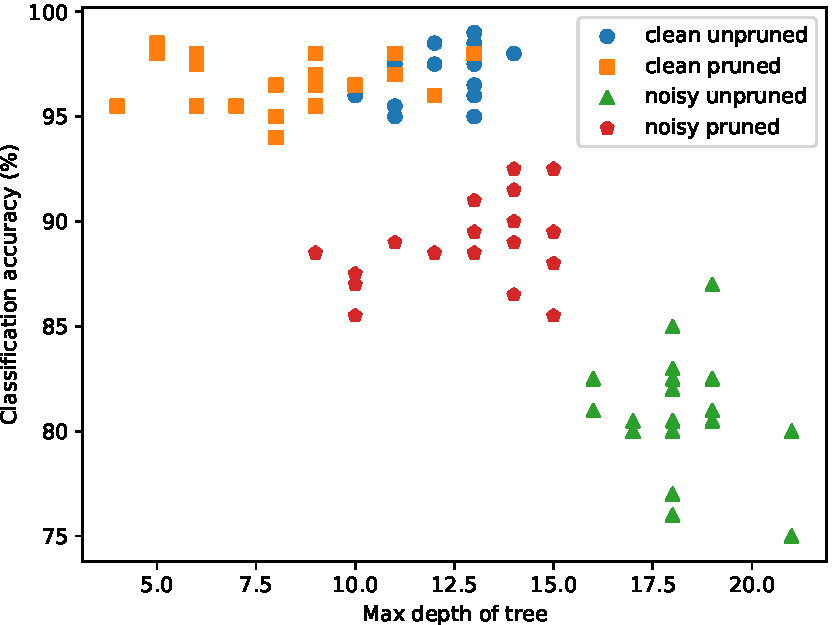
\includegraphics[width=0.8\textwidth]{figures/depth_plot.pdf}
    \caption{Classification accuracy against the maximum depth of the trees.}
    \label{fig:depth}
\end{subfigure}%
\begin{subfigure}[b]{.6\textwidth}
    \centering
    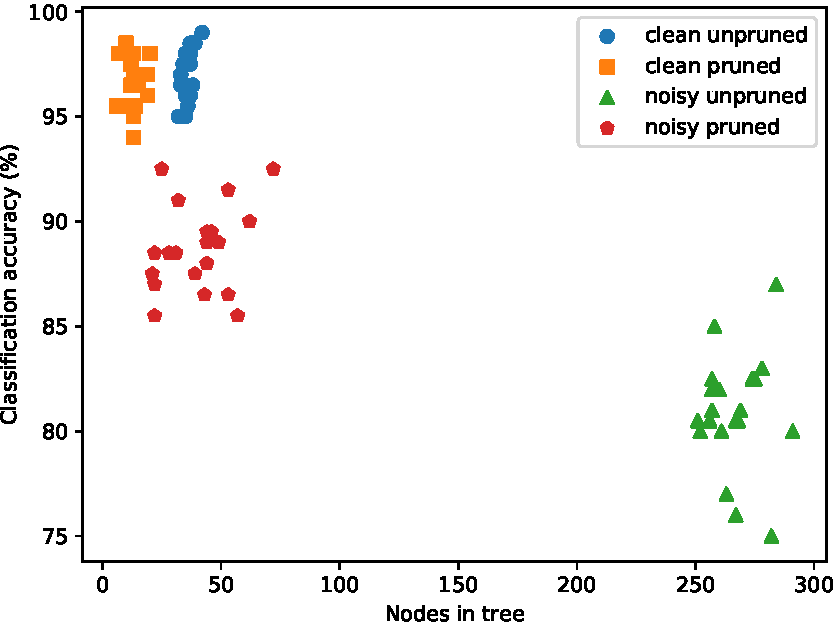
\includegraphics[width=0.8\textwidth]{figures/nodes_plot.pdf}
    \caption{Classification accuracy against the number of nodes in the trees.}
    \label{fig:nodes}
    \end{subfigure}%
}
\caption[Effects of Pruning on Depth and Sparseness]{The effects of pruning on max tree depth and the number of nodes in the tree (both excluding leaves), and how these correlate with classification accuracy. In both plots, 20 trees were trained then tested before and after pruning.}
\label{fig:pruning_effect_overview}
\end{figure}
%
From \autoref{fig:depth} we may be tempted to infer a negative correlation between the max depth and classification accuracy, however, this only holds for the case of the noisy dataset. Indeed, in the context of noisy data such a relationship is to be expected as pruning helps to reduce meaningless overfitting. Conversely, for a pristine dataset, the tree should only extract meaningful relationships, and thus reach a depth similar to the optimal one.
% The main point should be when there is noise in the dataset, as the trees are likely to overfit to the noise leading to deeper trees when unconstrained, which in turn lead to lower classification rates on average.

Additionally, we considered the impact of imposing a "maximum\_depth" hyperparameter on the model, capping the maximum depth of the tree. We observed that for shallow trees (maximum\_depth of 2 or below), increasing the maximum\_depth improved the classification rate. This is expected as this threshold prevents the tree from learning the underlying distribution of the data, so model performance suffers. However, increasing this threshold further (using the noisy dataset), overfitting starts to take over so the classification accuracy falls again, and in the case of the clean dataset there are no meaningful splits left to make. Therefore, we conclude that the relationship between maximum depth and classification accuracy begins positive, for all cases, but plateaus and turns negative in some cases as max depth rises due to overfitting.
% The two main points should be 1) higher information gain higher up in the tree 2) shallow trees perform better due to susceptibility of decision trees to overfit.






% ==================================================== %
%% APPENDICES -----------------------------------------%
% ==================================================== %
\newpage
\begin{appendices}
\addtocontents{toc}{\protect\setcounter{tocdepth}{0}}
\section{Decision Tree Pruning}

\label{app:tree_figure}
\subsection{Clean Dataset}
\addtocontents{toc}{\protect\setcounter{tocdepth}{1}}
Here we demonstrate the effect of pruning on a decision tree trained on 1800 samples of the clean data set, and pruned on the remaining 200. For the sake of clarity in the visualization, the tree depth was capped at 5.\footnote{These visualizations were using the Visualizer class which we implemented.}
\begin{figure}[H]
    \centering
    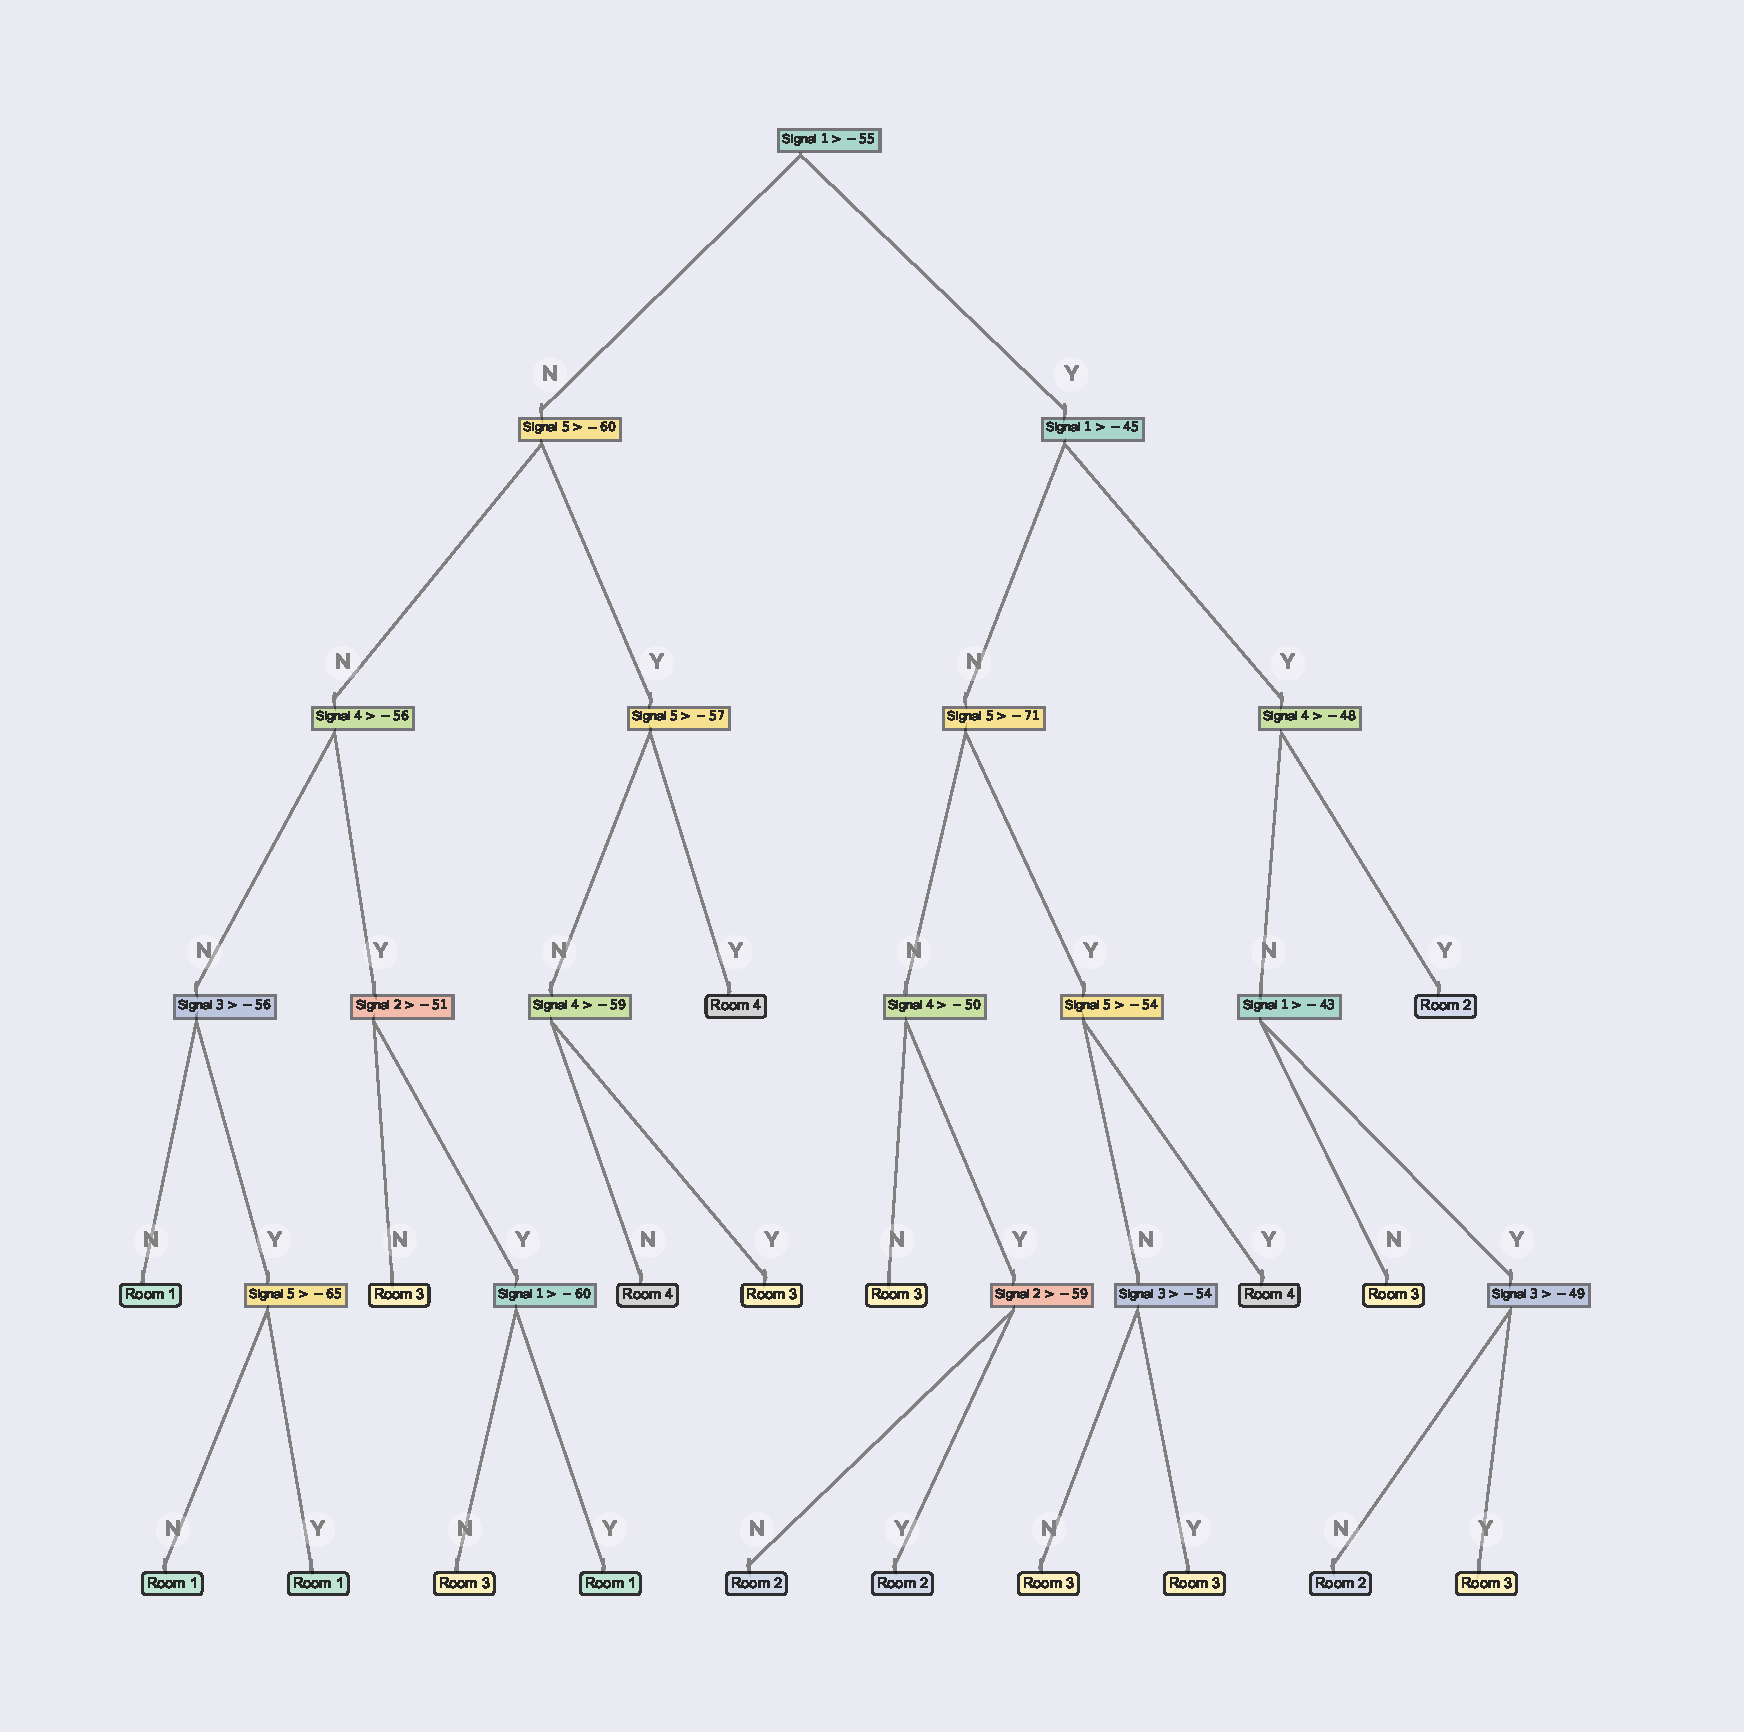
\includegraphics[width=\textwidth]{figures/clean_unpruned.pdf}
    \caption[Unpruned Tree for the Clean Dataset]{Resulting unpruned tree for the clean dataset}
    \label{fig:pruning_example_clean_unpruned}
\end{figure}

\newpage

\begin{figure}[H]
    \centering
    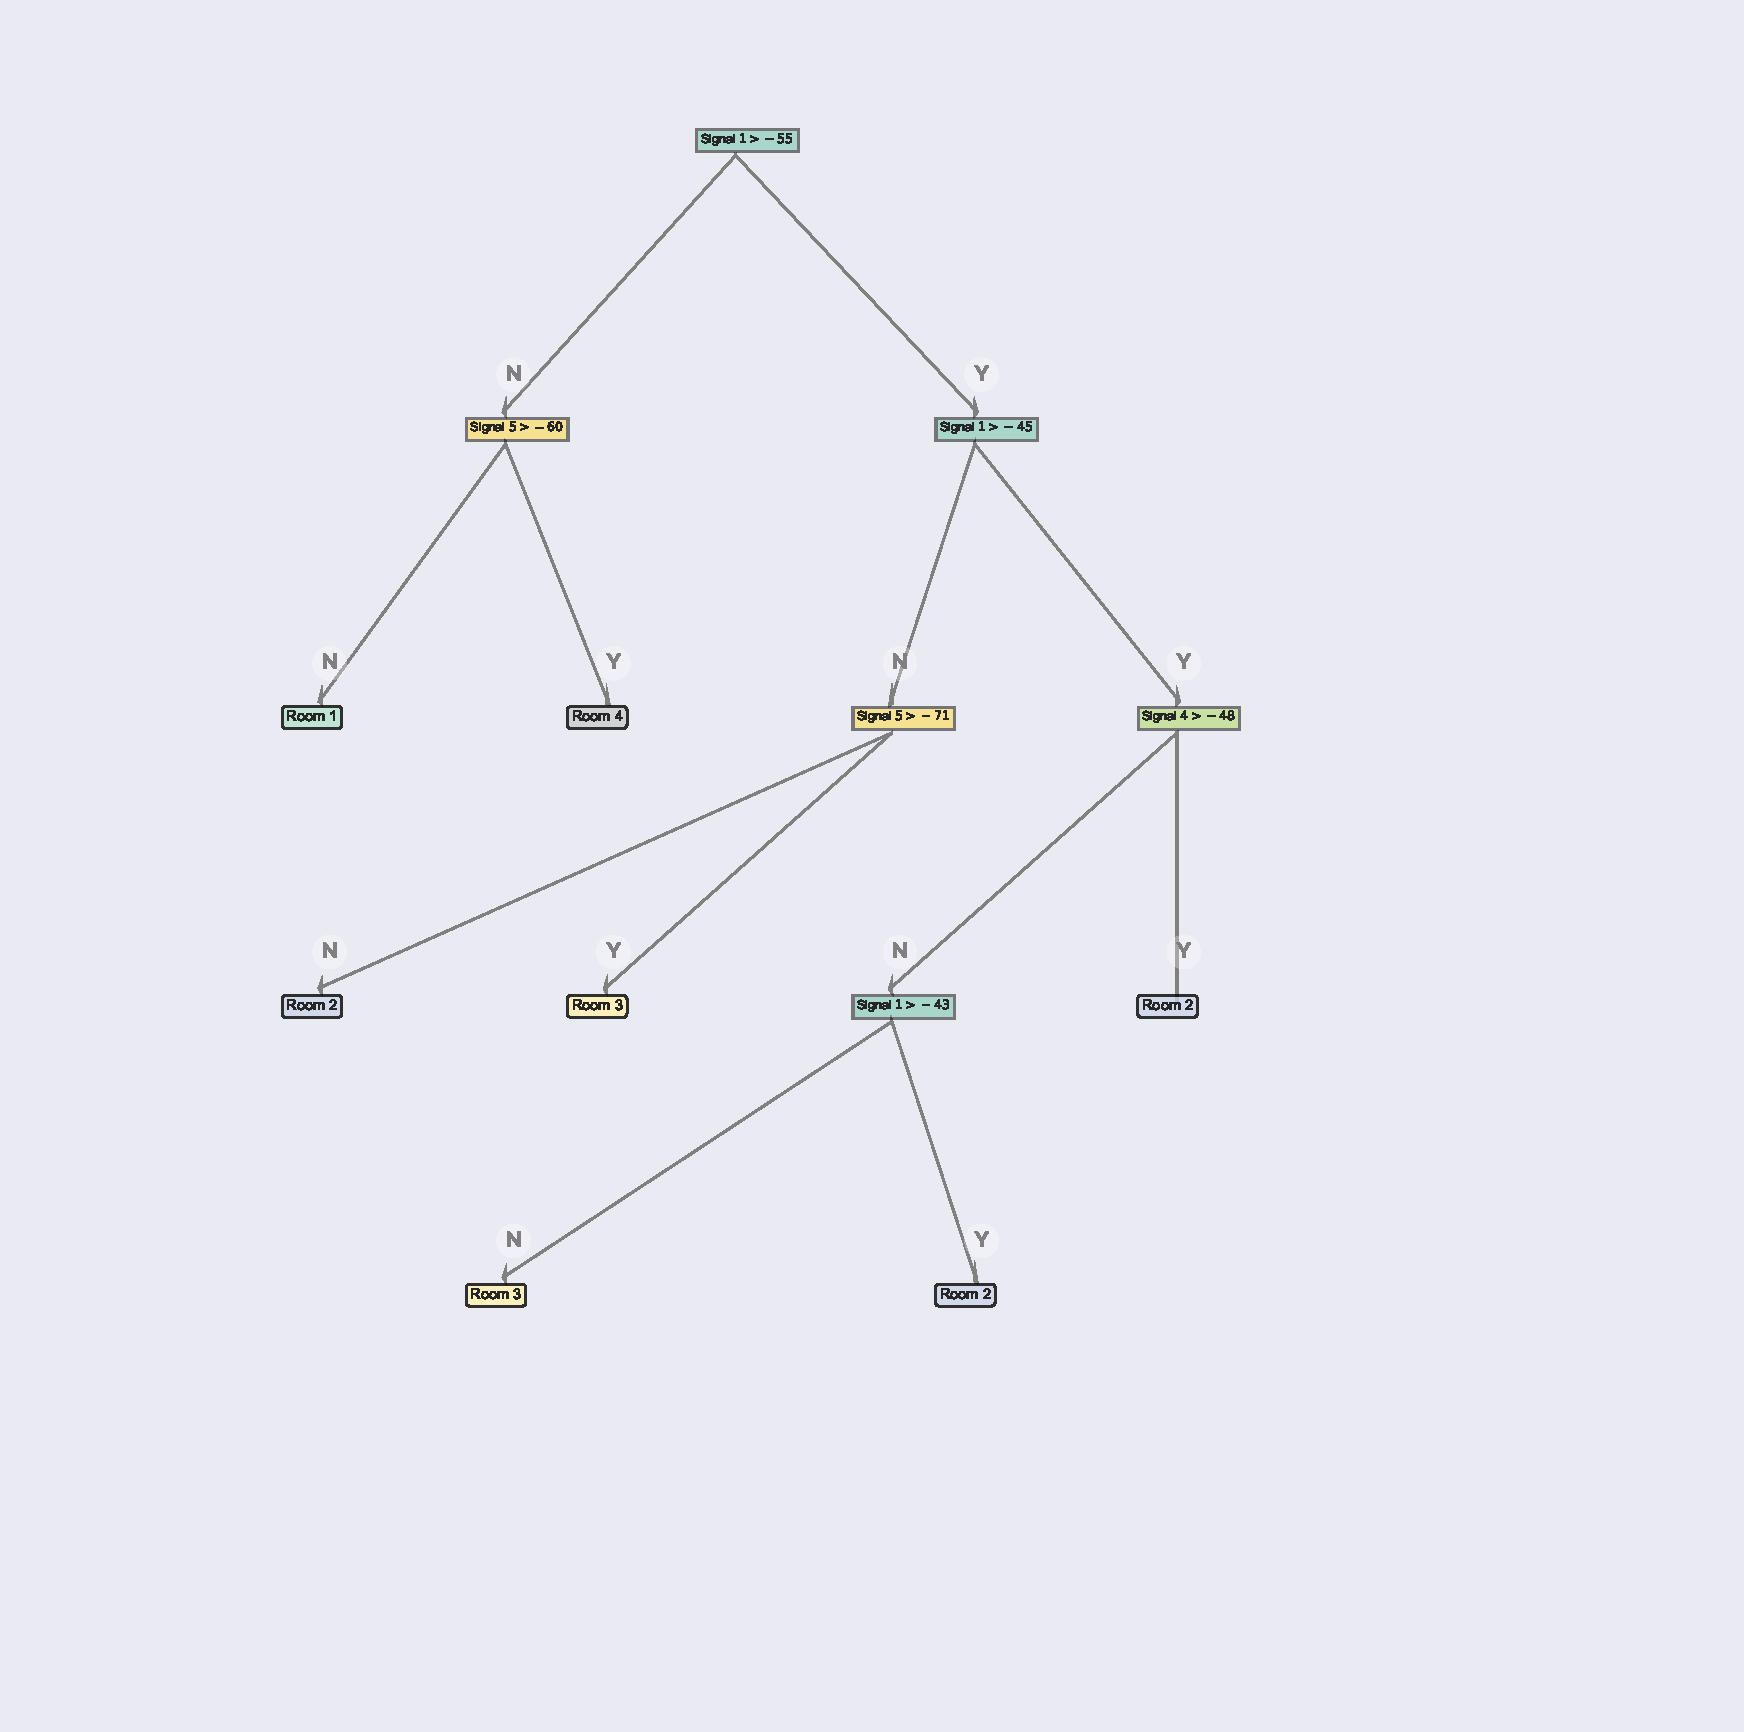
\includegraphics[width=\textwidth]{figures/clean_pruned.pdf}
    \caption[Pruned Tree for the Clean Dataset]{Resulting pruned tree for the clean dataset}
      \label{fig:pruning_example_clean_pruned}
\end{figure}
\newpage

\subsection{Noisy Dataset}
Here we demonstrate the effect of pruning on a decision tree trained on 1800 samples of the noisy data set, and pruned on the remaining 200. For the sake of clarity in the visualization, the tree depth was capped at 5.\footnote{These visualizations are automatically generated by the Visualizer class which we implemented}
\begin{figure}[H]
    \centering
    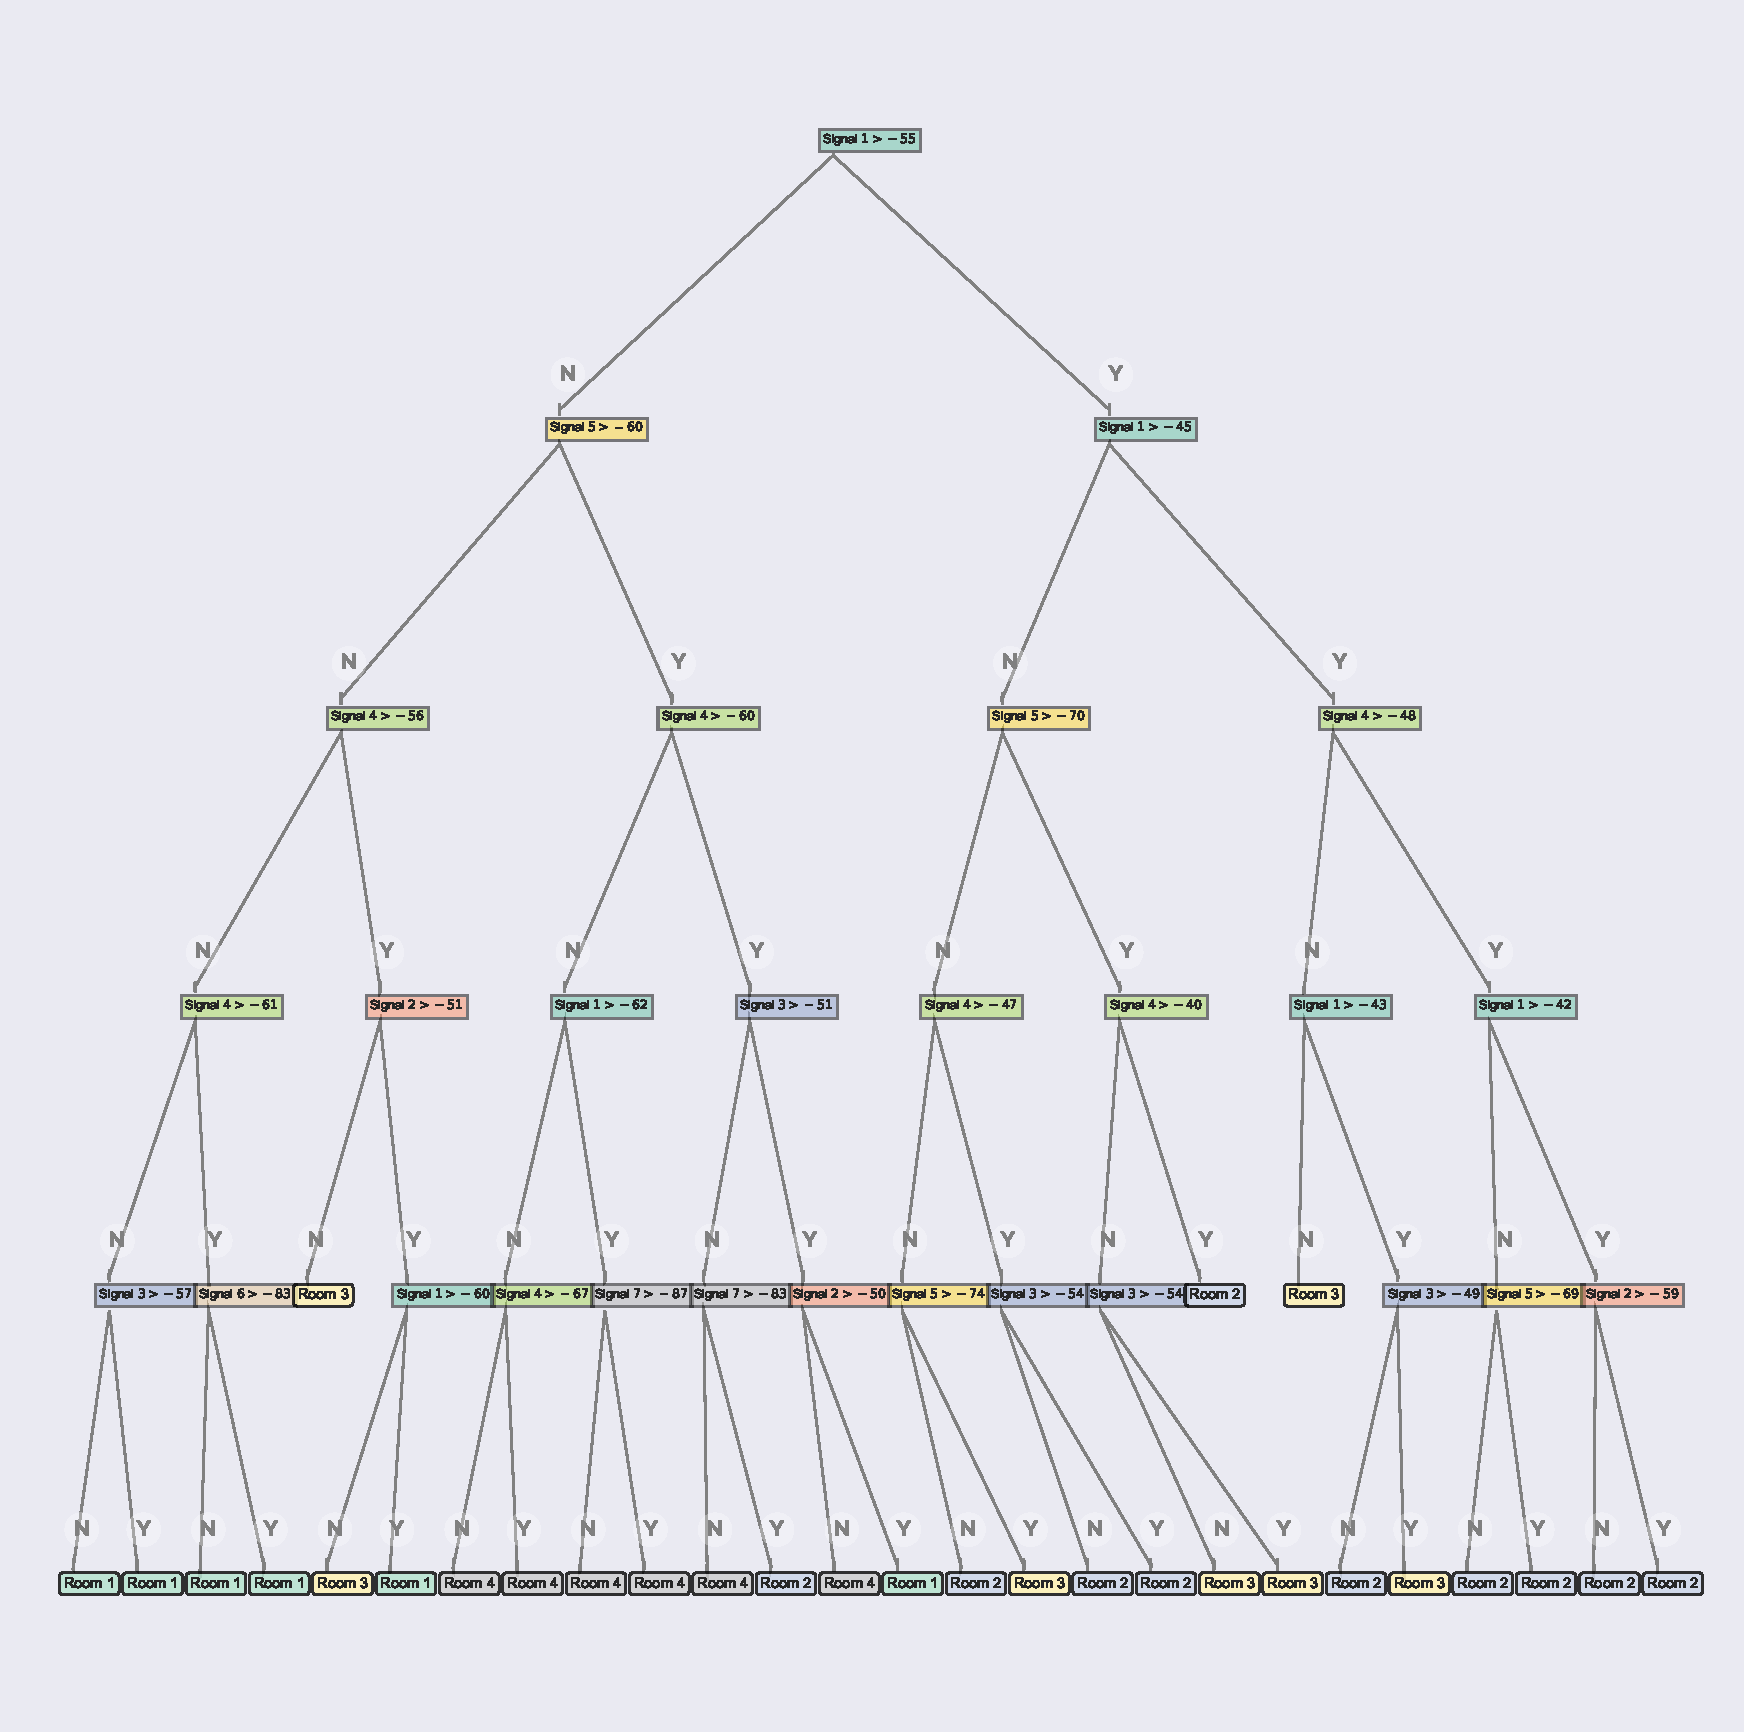
\includegraphics[width=\textwidth]{figures/noisy_unpruned.pdf}
    \caption[Unpruned Tree for the Noisy Dataset]{Resulting unpruned tree for the noisy dataset}
    \label{fig:pruning_example_noisy_unpruned}
\end{figure}

\newpage

\begin{figure}[H]
    \centering
    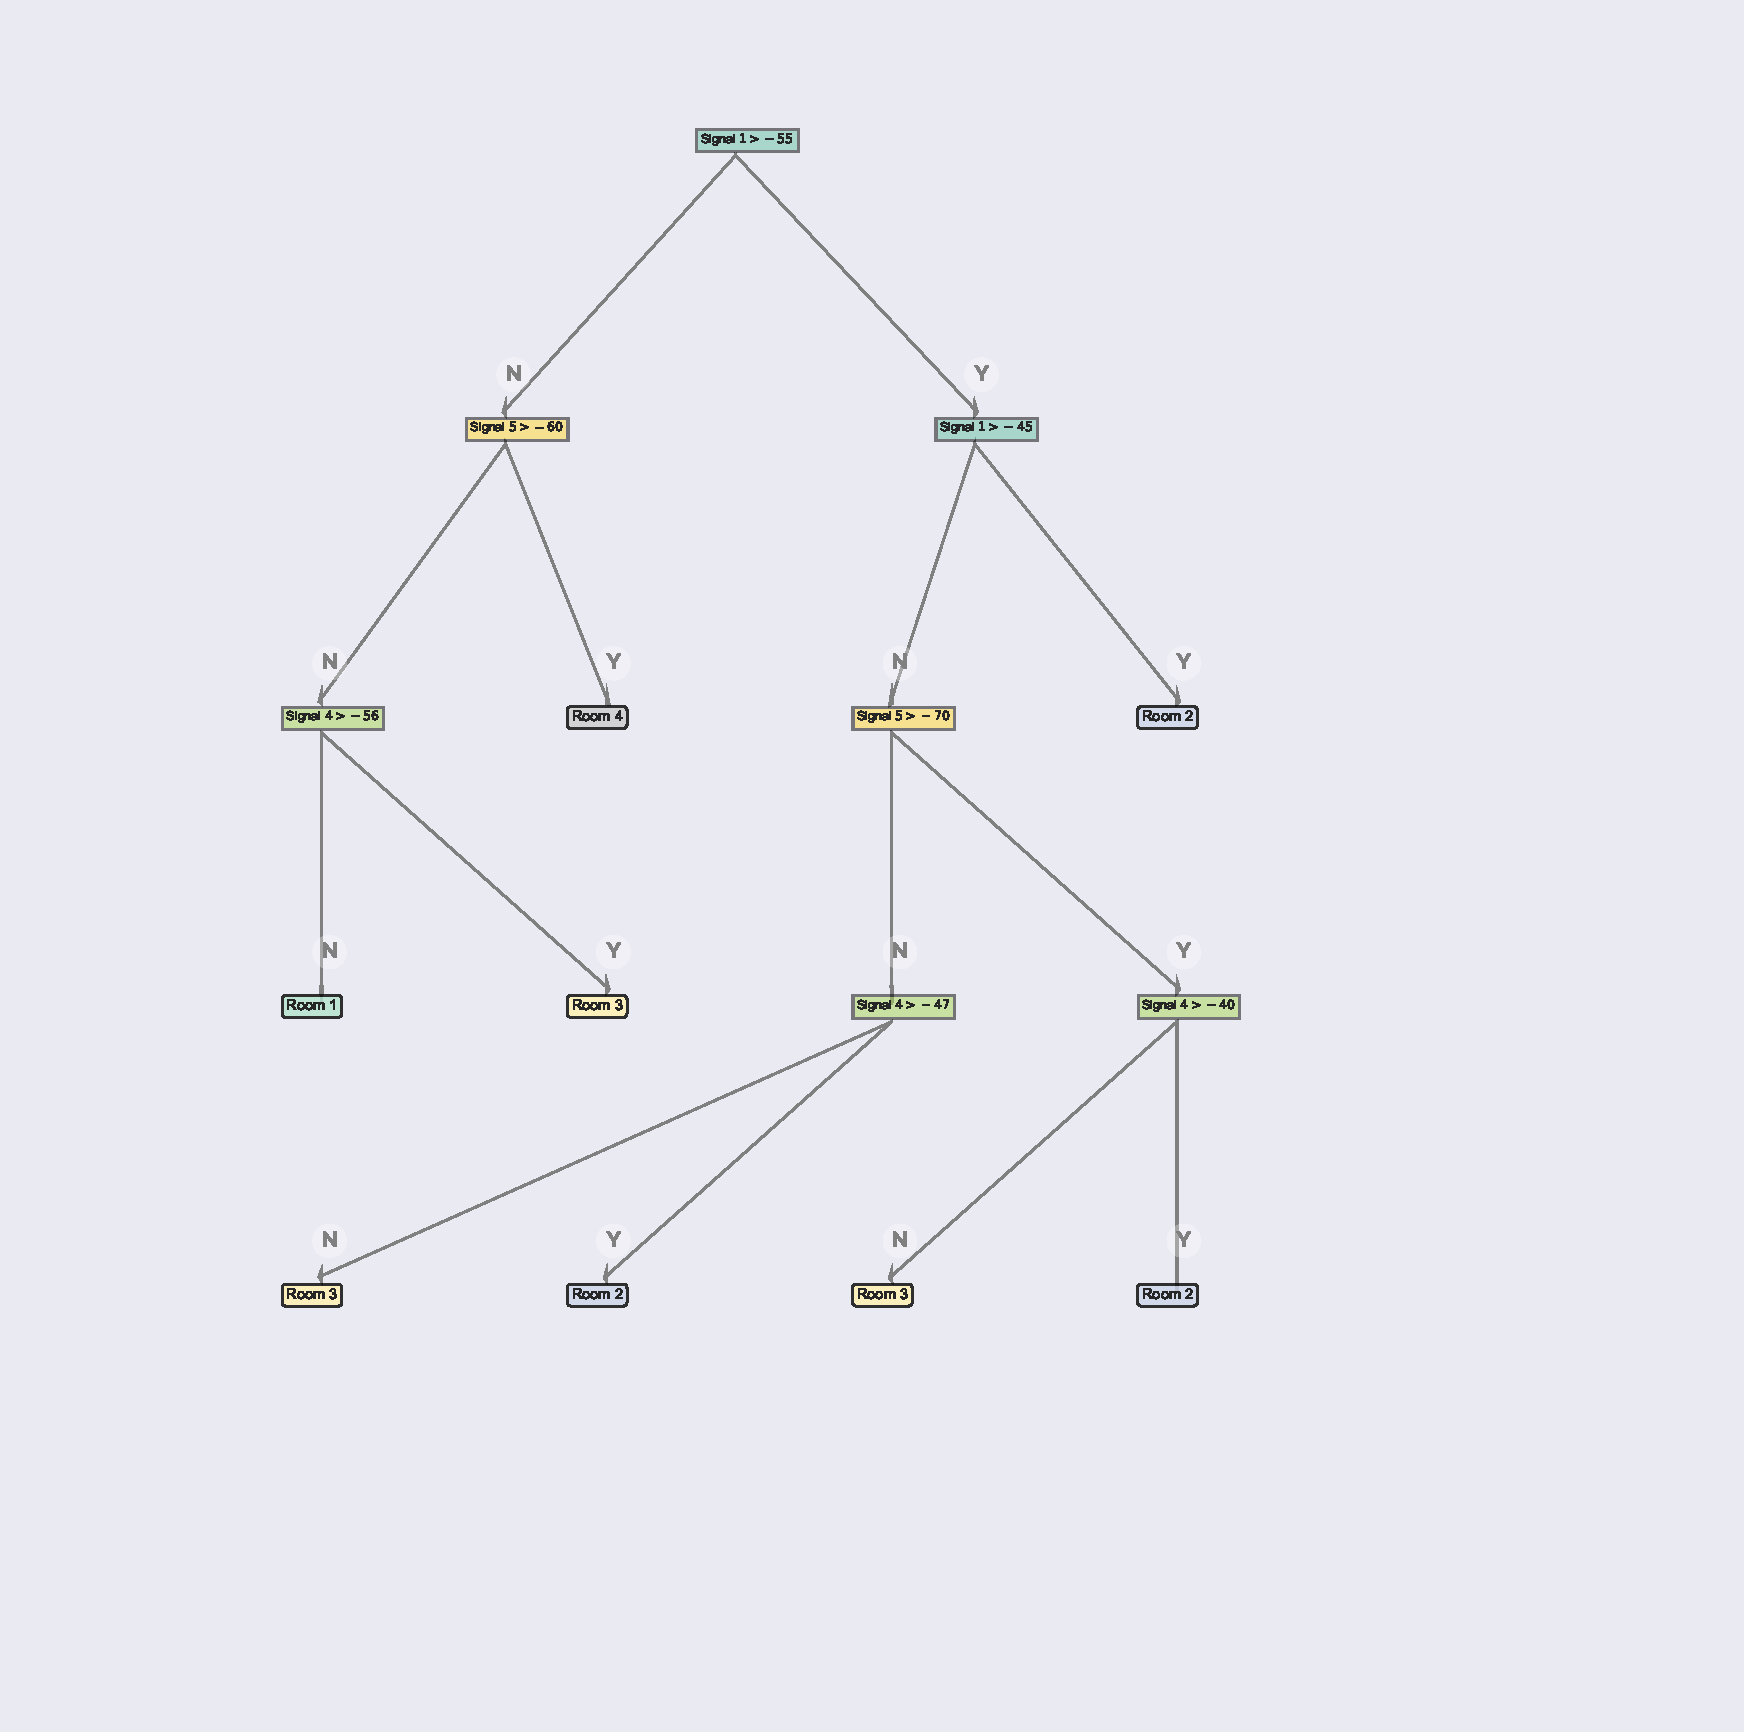
\includegraphics[width=\textwidth]{figures/noisy_pruned.pdf}
    \caption[Pruned Tree for the Noisy Dataset]{Resulting pruned tree for the noisy dataset}
      \label{fig:pruning_example_noisy_pruned}
\end{figure}
% \begin{figure}[h!]
% \centering
% 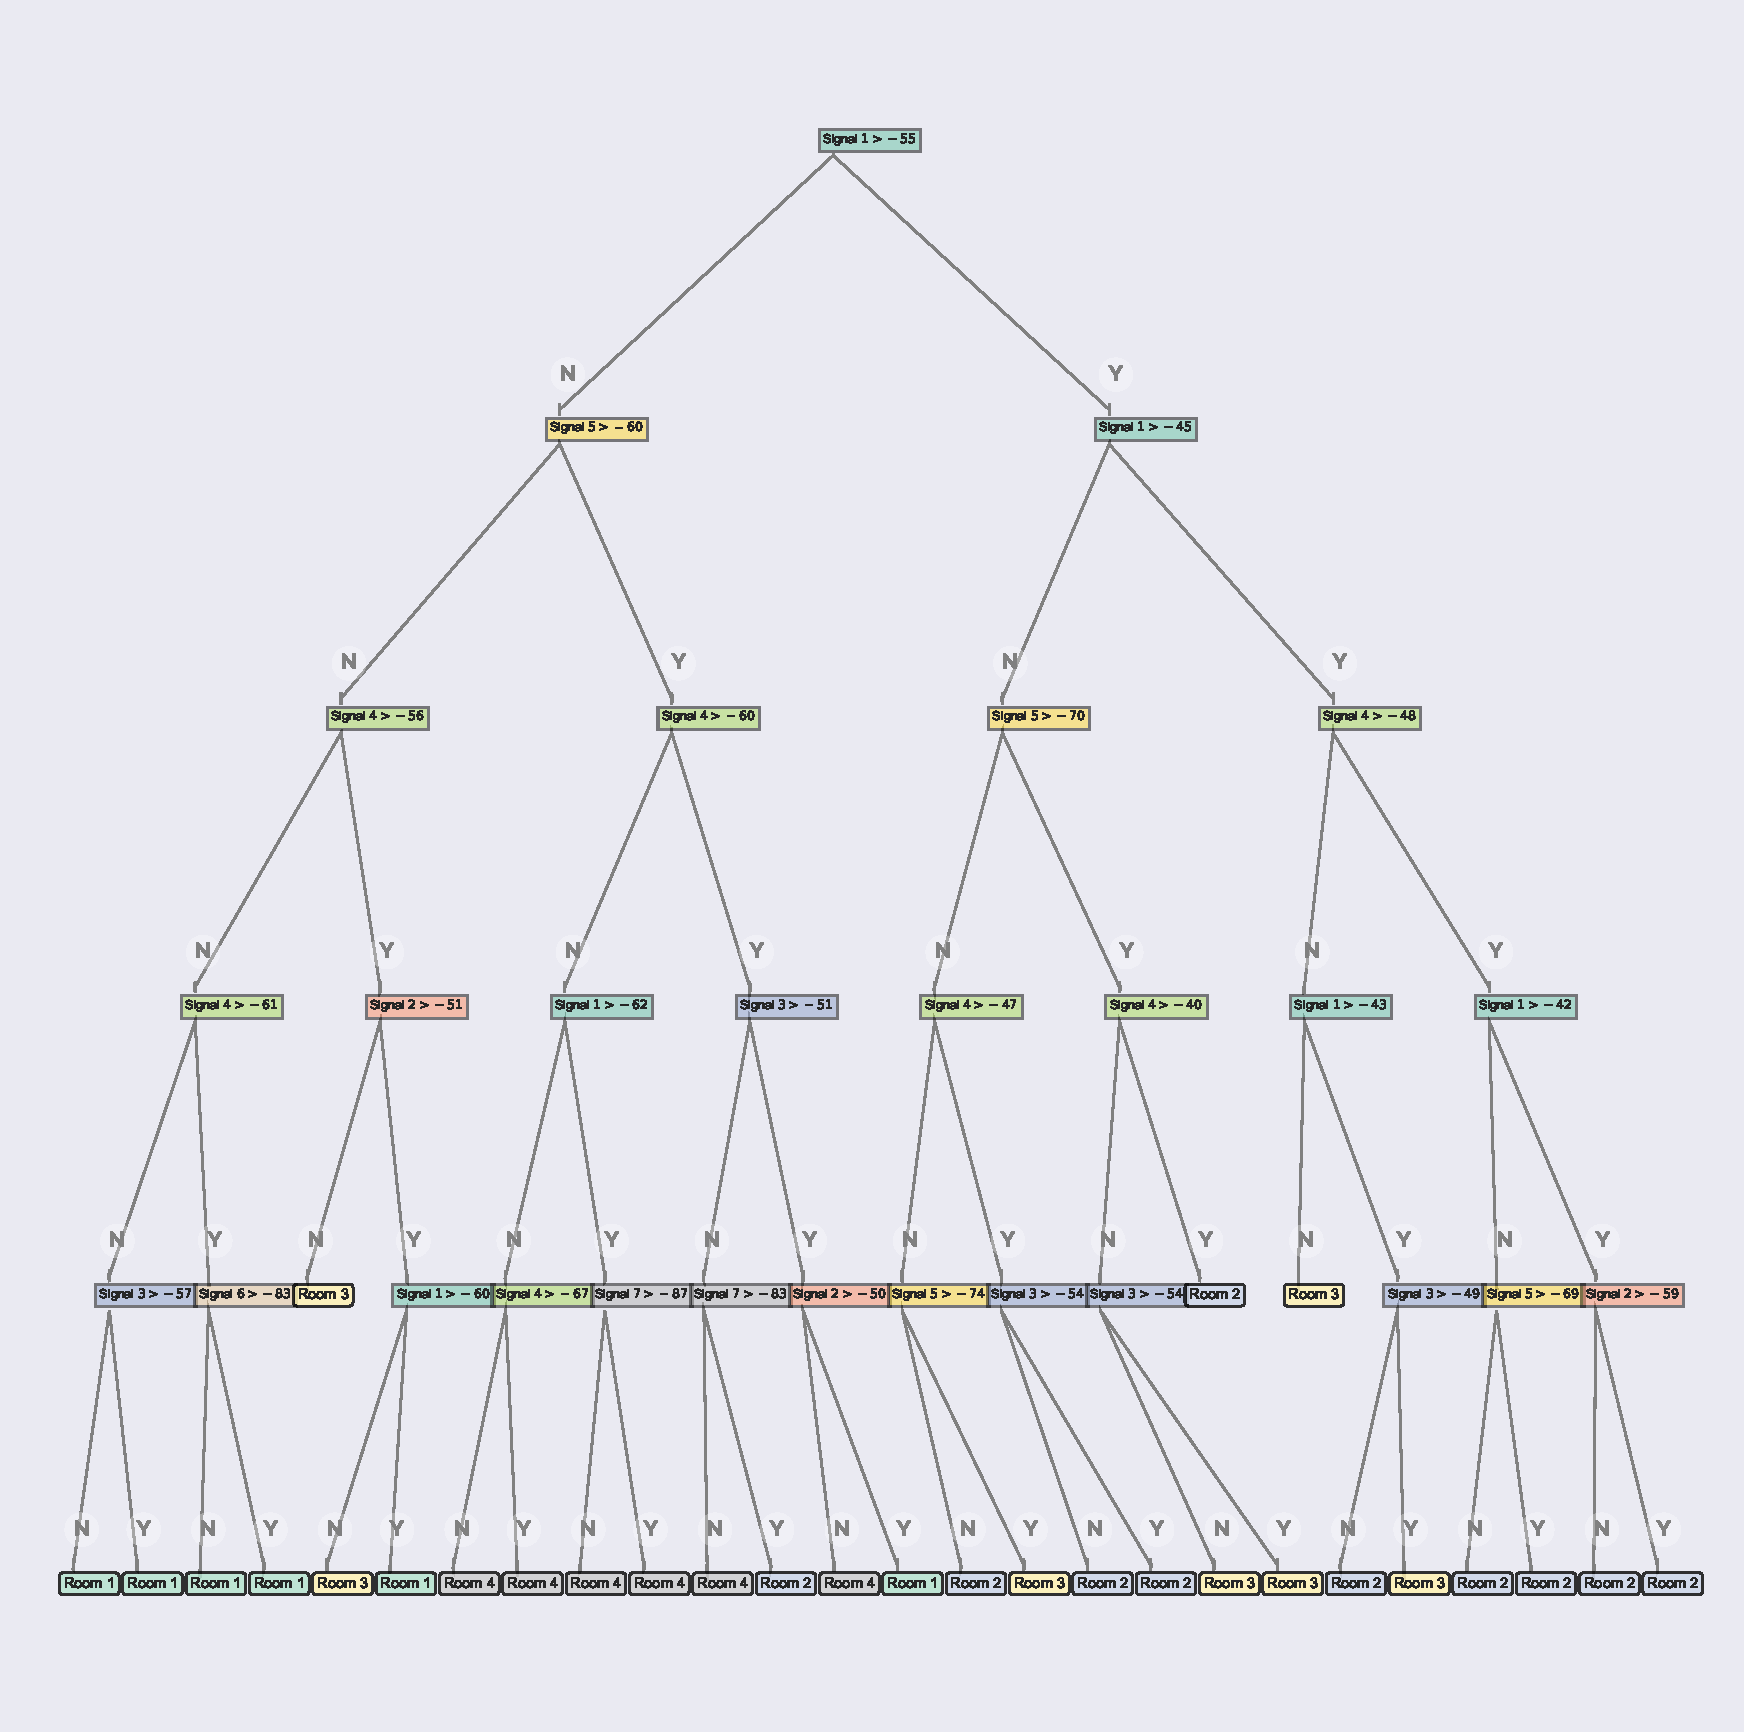
\includegraphics[width=0.65\textwidth]{figures/noisy_unpruned.pdf}
% 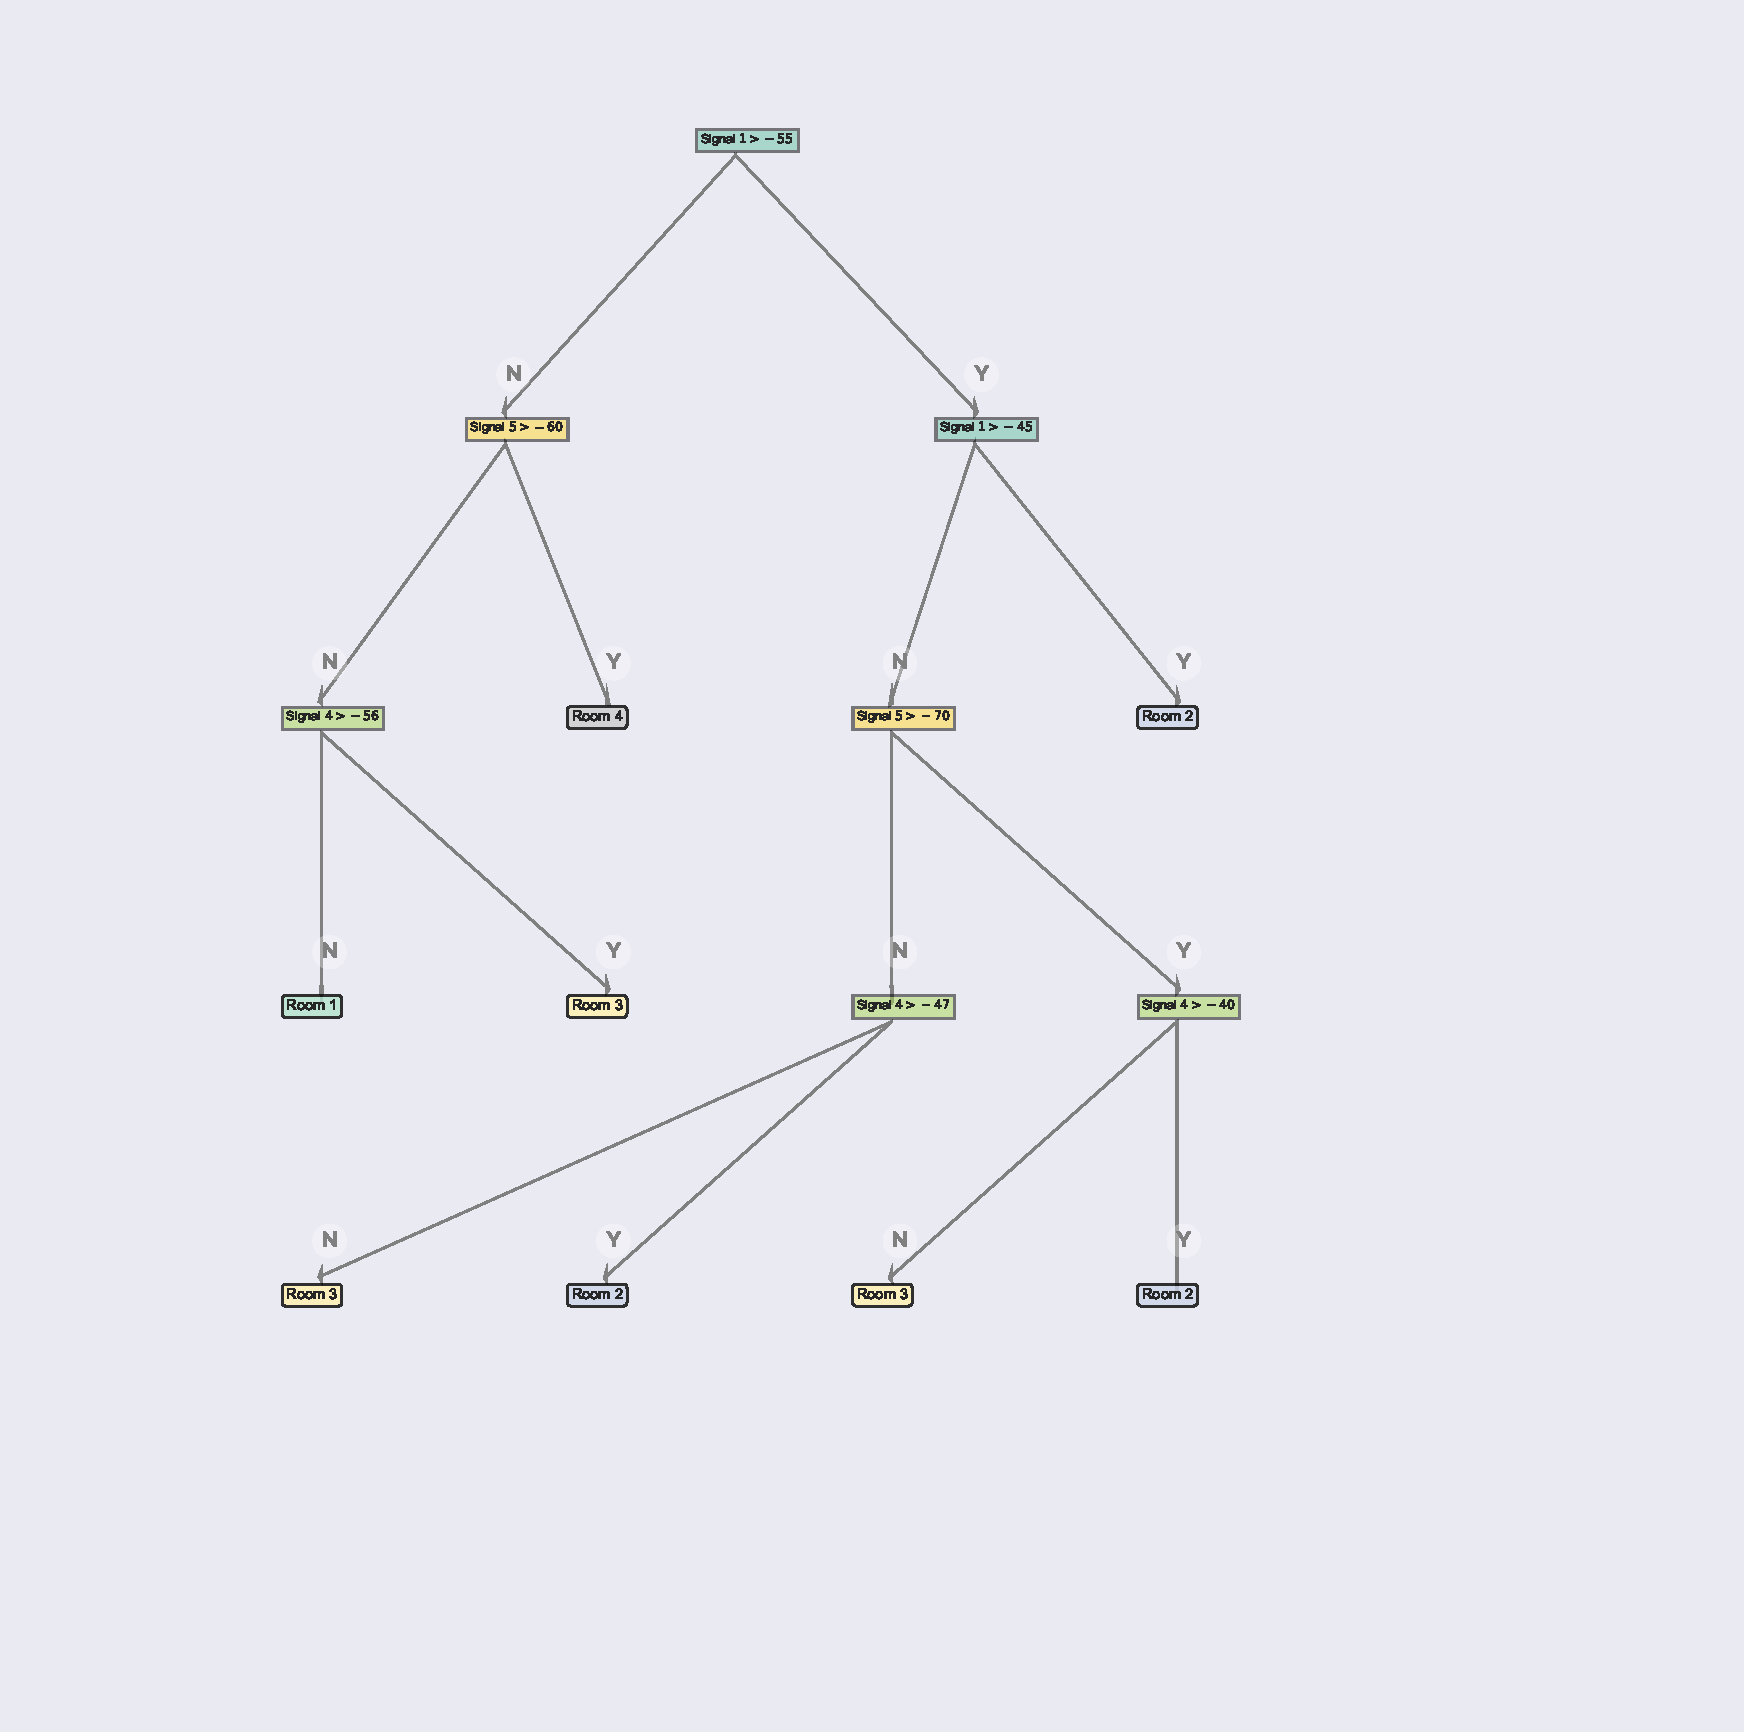
\includegraphics[width=0.65\textwidth]{figures/noisy_pruned.pdf}
% \caption{Here we demonstrate the effect of pruning on a decision tree trained on 1800 samples of the noisy data set, and pruned on the remaining 200. For the sake of clarity in the visualization, the tree depth was capped at 5.\footnote{These visualizations are automatically generated by the Visualizer class which we implemented.}}
% \
% \end{figure}
\newpage
\subsection{Entire Dataset}
Here we demonstrate the effect of pruning on a decision tree trained on 3600 samples of the total data set, and pruned on the remaining 400. The tree depth was not capped. 
\begin{figure}[H]
    \centering
    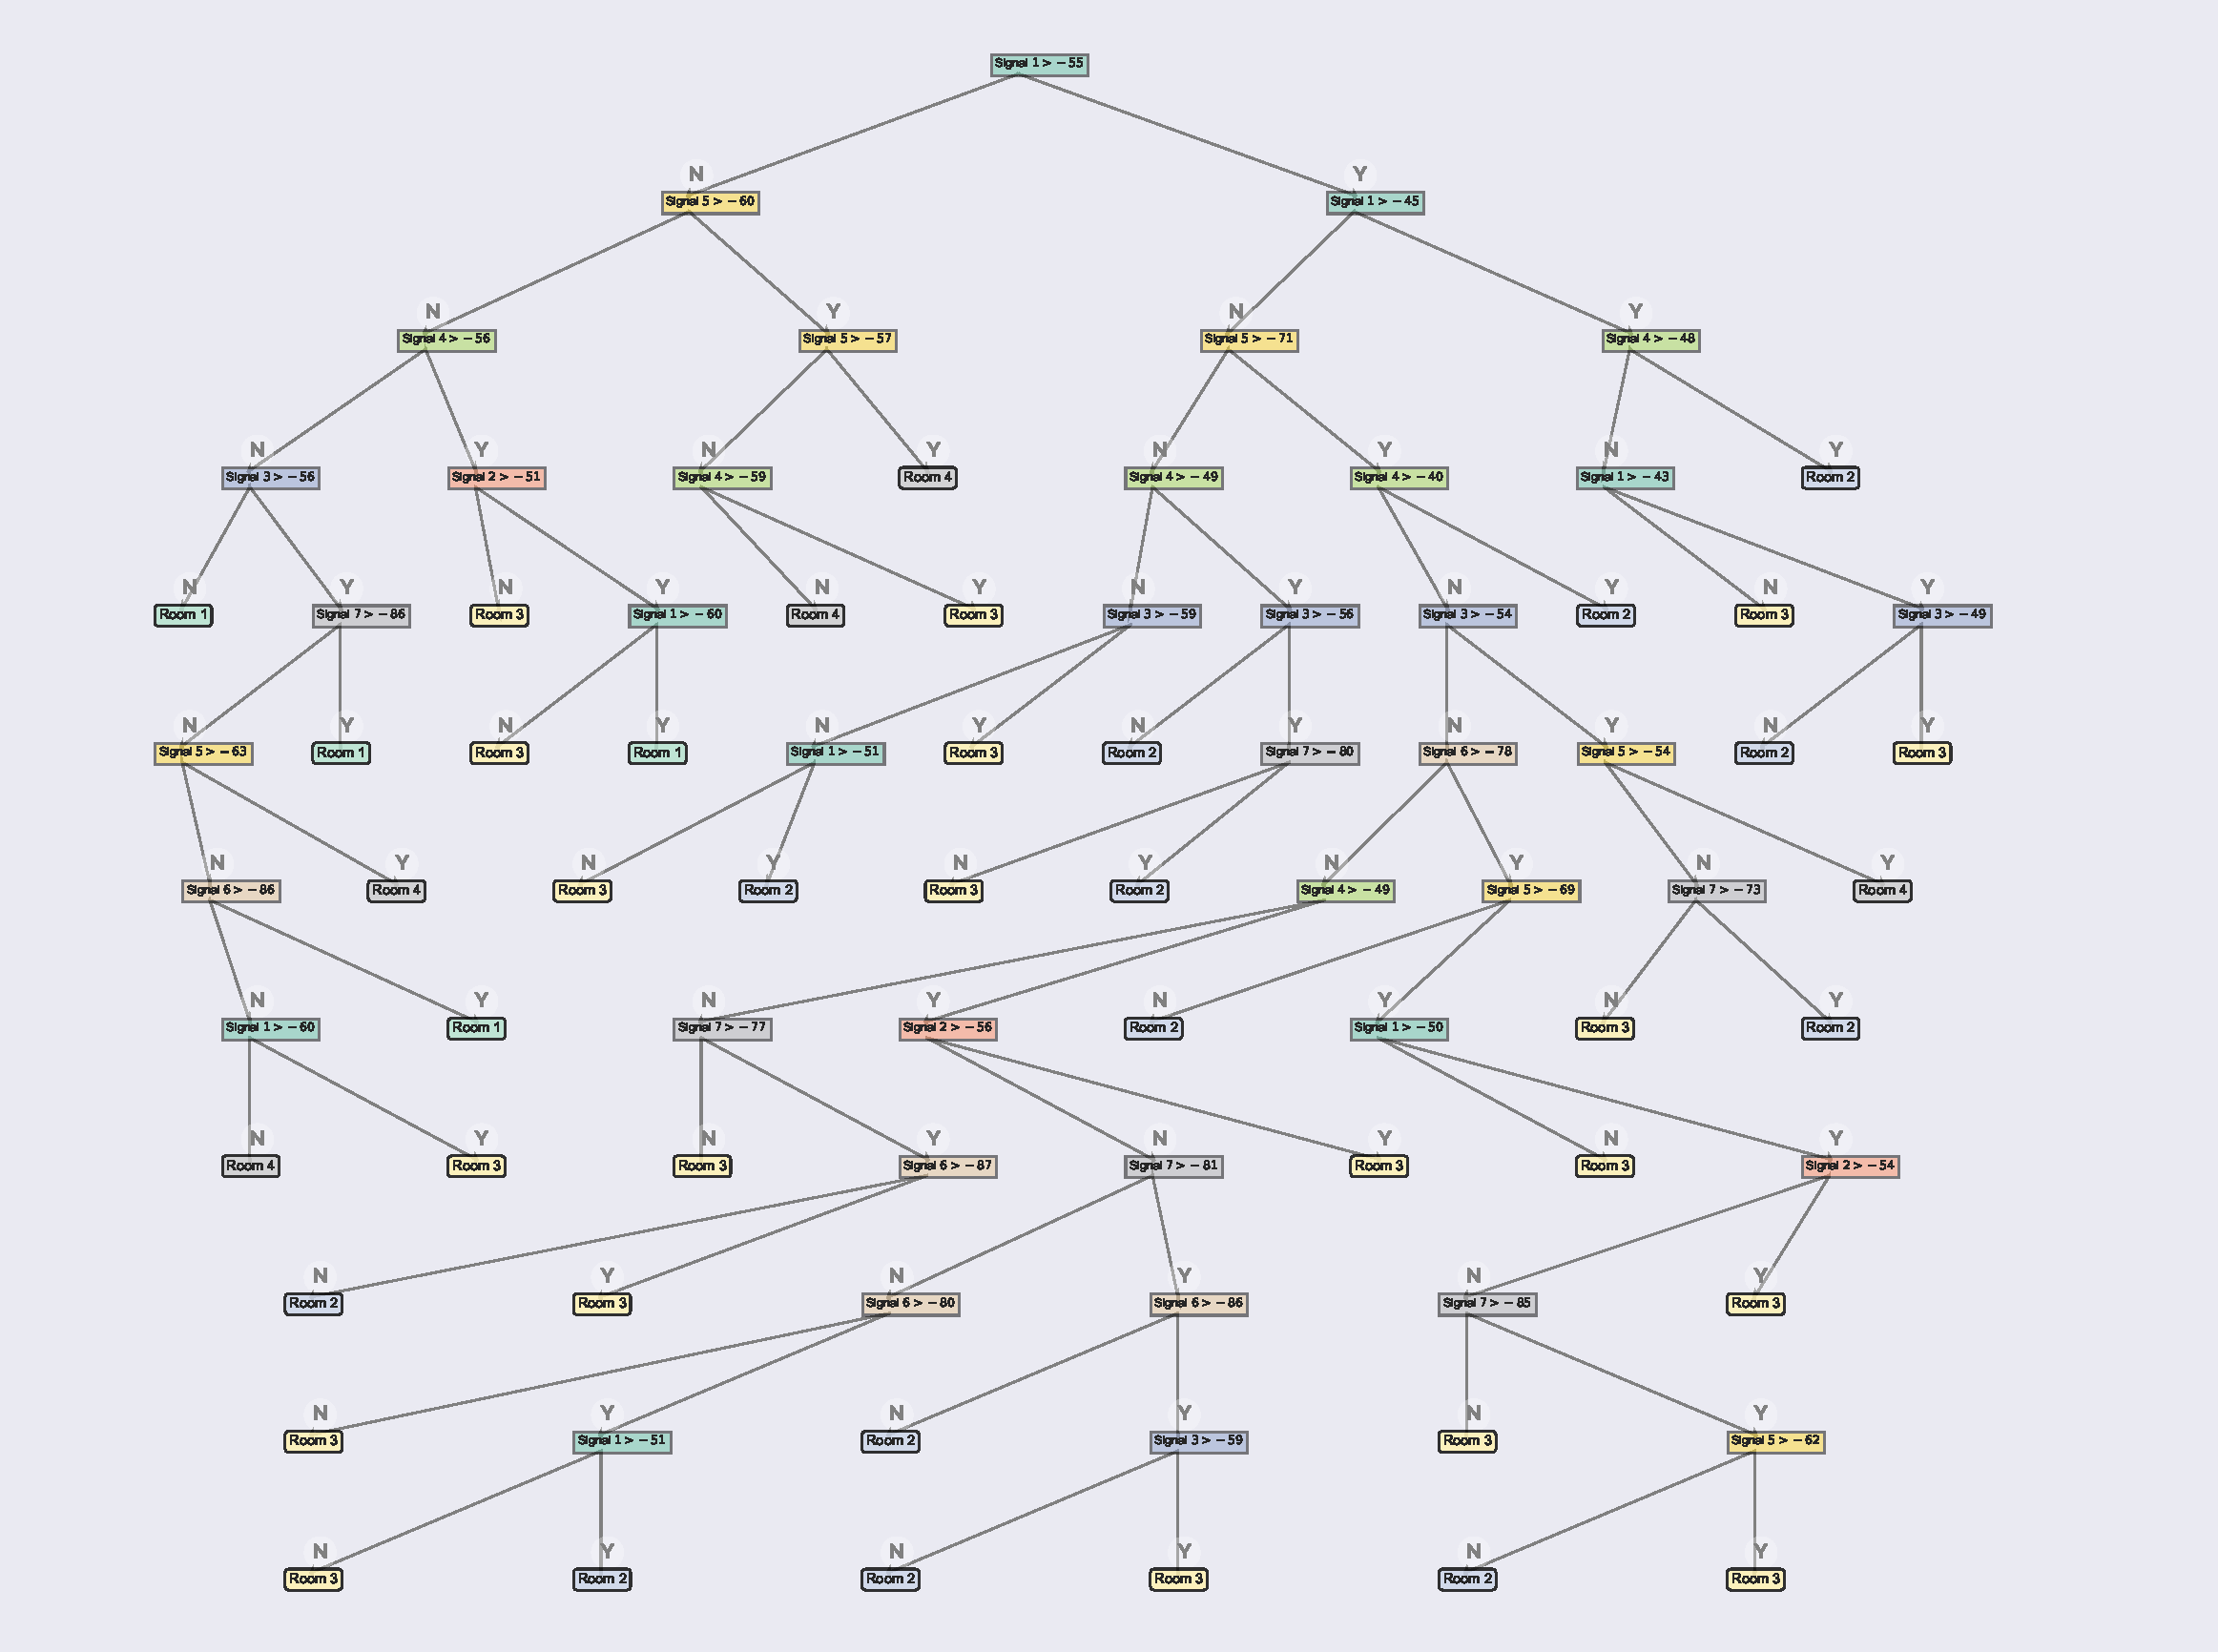
\includegraphics[width=\textwidth]{figures/total_unpruned.pdf}
    \caption[Unpruned Tree for the Entire Dataset]{Resulting unpruned tree for the entire dataset}
    \label{fig:pruning_example_total_unpruned}
\end{figure}

\newpage
\begin{figure}[H]
    \centering
    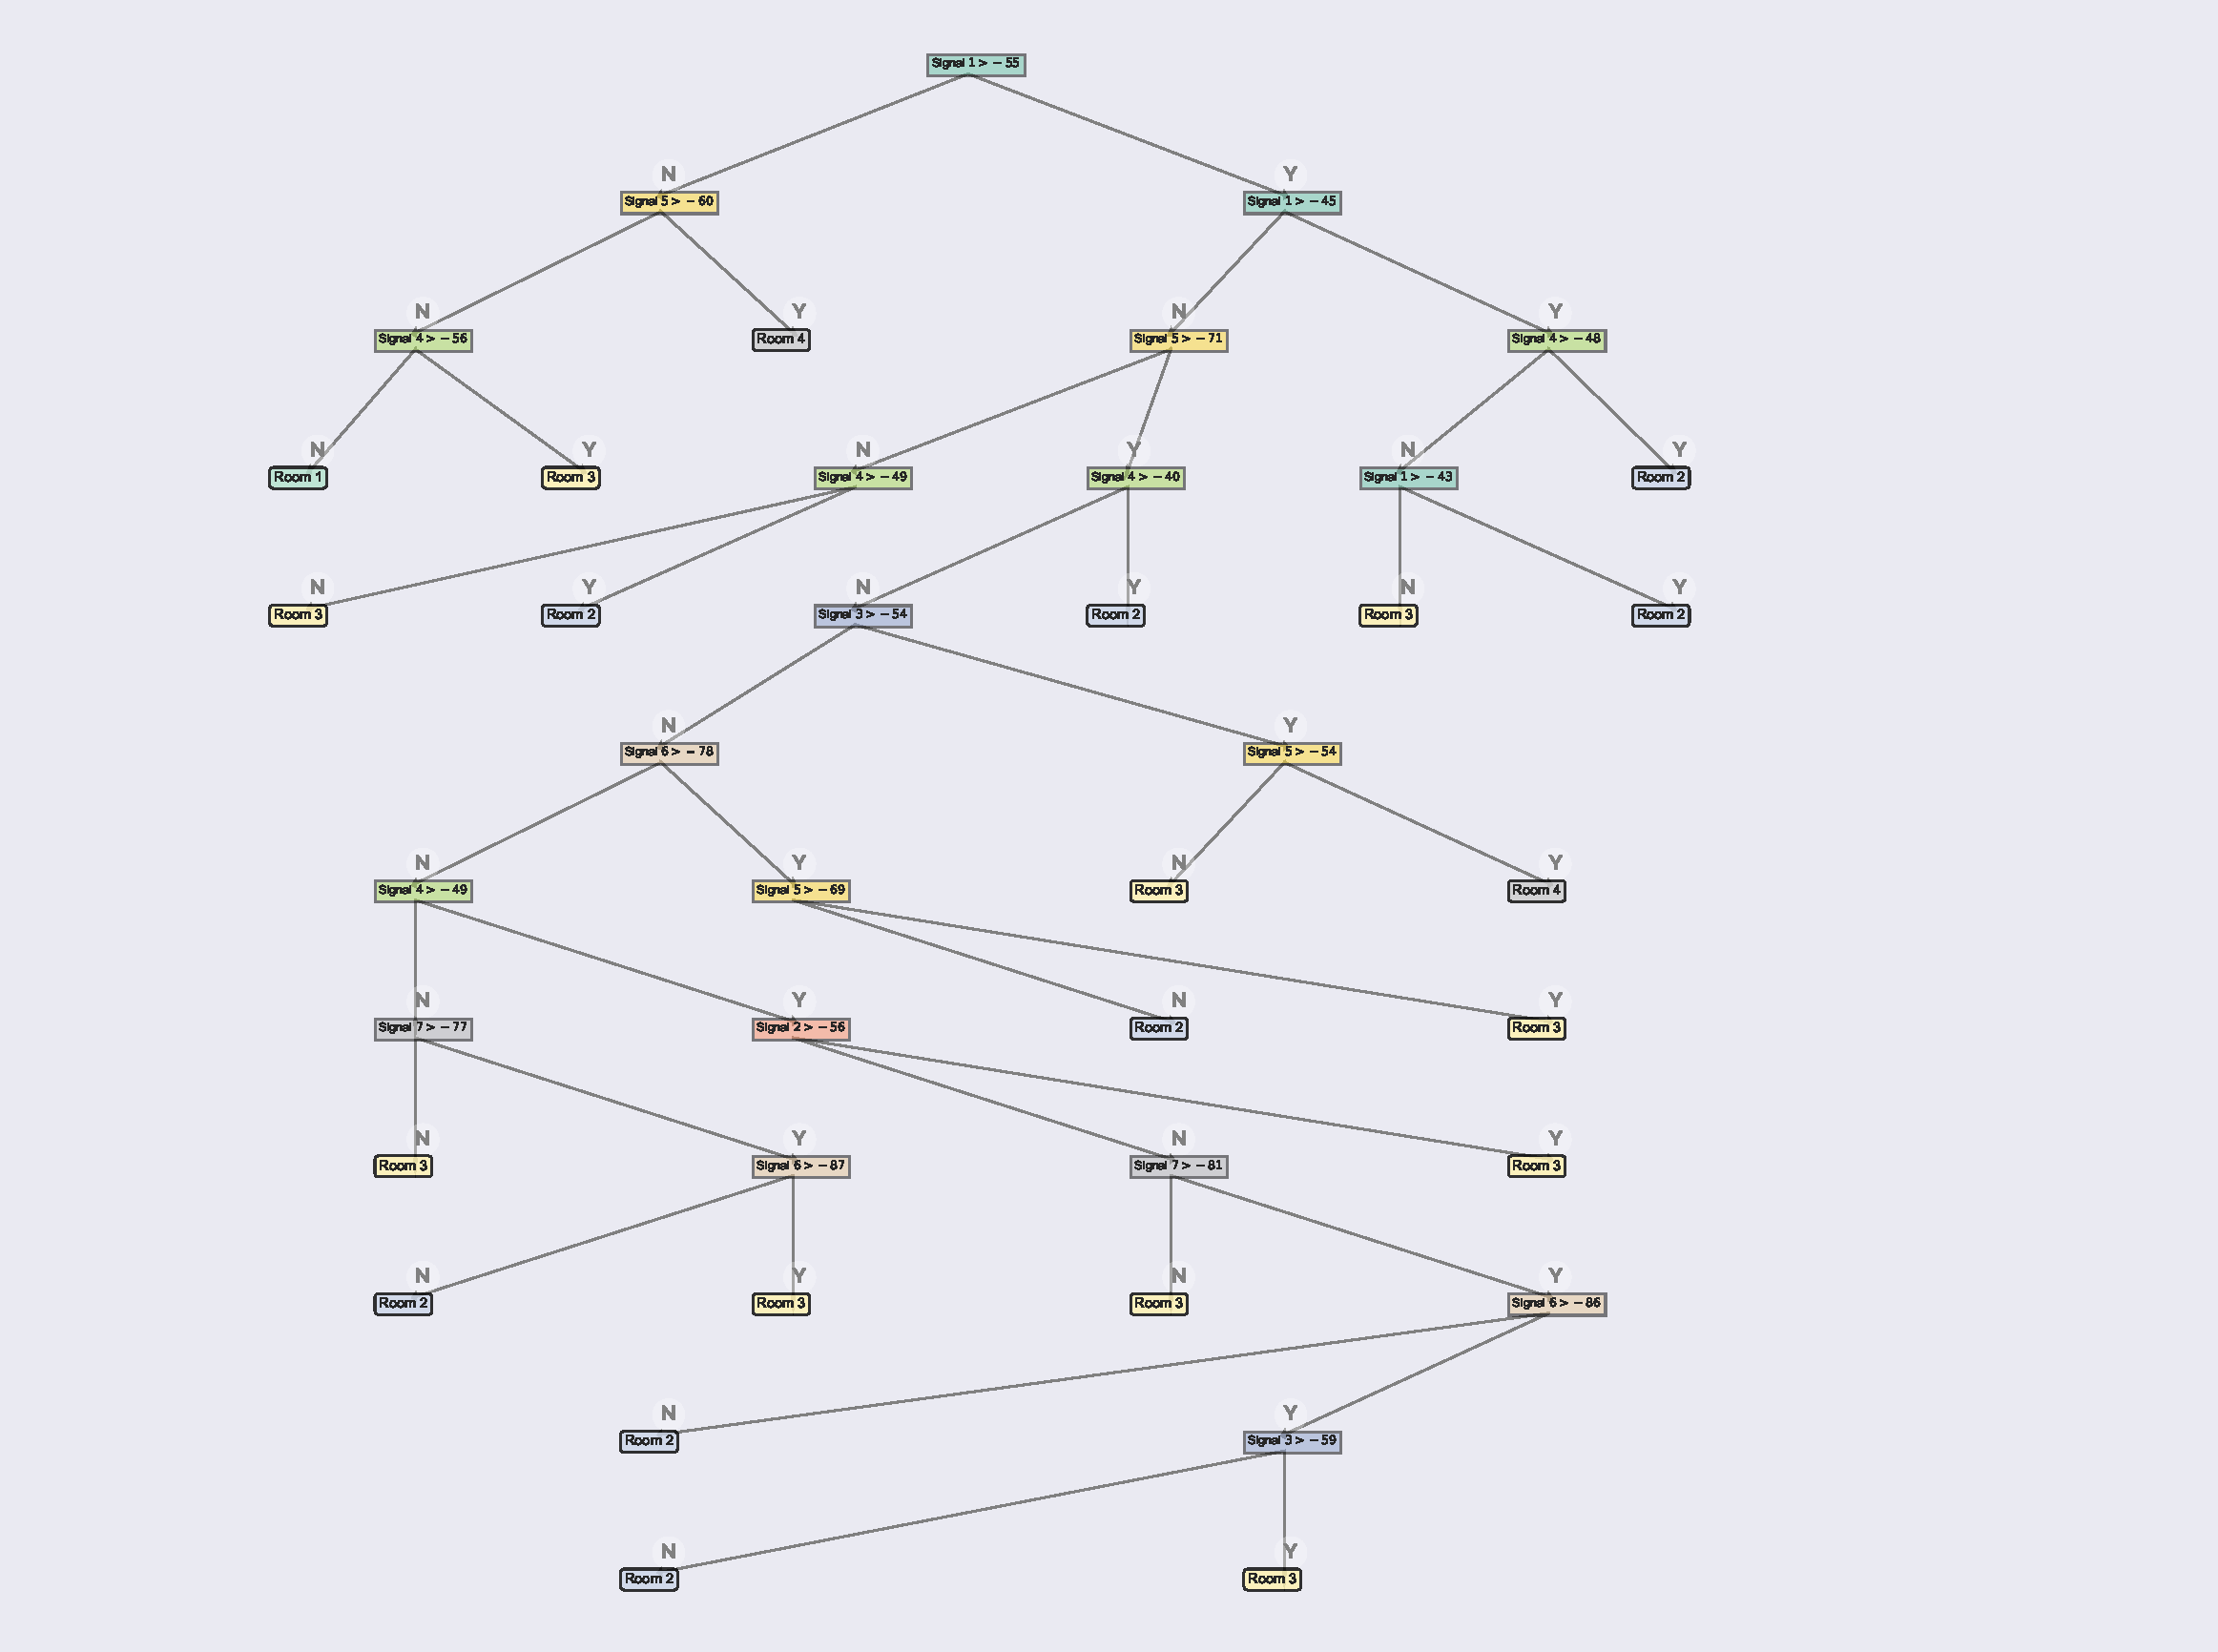
\includegraphics[width=\textwidth]{figures/total_pruned.pdf}
    \caption[Pruned Tree for the Entire Dataset]{Resulting pruned tree for the entire dataset}
      \label{fig:pruning_example_total_pruned}
\end{figure}
\newpage
\addtocontents{toc}{\protect\setcounter{tocdepth}{0}}
\section{Tables}
\label{app:results}
\addtocontents{toc}{\protect\setcounter{tocdepth}{1}}
\subsection{Unpruned Clean:} \\ 
\label{sec:data_unpruned_clean}
\begin{table}[H]
\small\addtolength{\tabcolsep}{-5pt}
\centering
\begin{tabular}{|
>{\columncolor[HTML]{EFEFEF}}l |l|l|l|l|}
\hline
                       & \cellcolor[HTML]{EFEFEF}\textbf{Room 1 Predicted} & \cellcolor[HTML]{EFEFEF}\textbf{Room 2 Predicted} & \cellcolor[HTML]{EFEFEF}\textbf{Room 3 Predicted} & \cellcolor[HTML]{EFEFEF}\textbf{Room 4 predicted} \\ \hline
\textbf{Room 1 Actual} & 0.986                                             & 0.000                                             & 0.006                                             & 0.008                                             \\ \hline
\textbf{Room 2 Actual} & 0.000                                             & 0.959                                             & 0.041                                             & 0.000                                             \\ \hline
\textbf{Room 3 Actual} & 0.001                                             & 0.044                                             & 0.949                                             & 0.006                                             \\ \hline
\textbf{Room 4 Actual} & 0.008                                             & 0.000                                             & 0.003                                             & 0.990                                             \\ \hline
\end{tabular}
\caption[Metrics for Clean Unpruned]{Unpruned clean confusion matrix}
\label{tab:confusion_clean_unpruned}
\end{table}

\begin{table}[H]
\small\addtolength{\tabcolsep}{-5pt}
\centering
\begin{tabular}{|l|l|l|l|l|}
\hline
\rowcolor[HTML]{EFEFEF} 
                                           & \textbf{Room 1} & \textbf{Room 2} & \textbf{Room 3} & \textbf{Room 4} \\ \hline
\cellcolor[HTML]{EFEFEF}\textbf{Recall}    & 0.986           & 0.959           & 0.949           & 0.990           \\ \hline
\cellcolor[HTML]{EFEFEF}\textbf{Precision} & 0.991           & 0.957           & 0.951           & 0.986           \\ \hline
\cellcolor[HTML]{EFEFEF}\textbf{F1}        & 0.988           & 0.958           & 0.950           & 0.988           \\ \hline
\end{tabular}
\caption[]{Average recall, precision and F1 for the unpruned clean dataset}
\label{tab:RPF_unpruned_clean}
\end{table}

\subsection{Pruned Clean:}
\label{sec:data_pruned_clean}

\begin{table}[H]
\small\addtolength{\tabcolsep}{-5pt}
\centering
\begin{tabular}{|
>{\columncolor[HTML]{EFEFEF}}l |l|l|l|l|}
\hline
                       & \cellcolor[HTML]{EFEFEF}\textbf{Room 1 Predicted} & \cellcolor[HTML]{EFEFEF}\textbf{Room 2 Predicted} & \cellcolor[HTML]{EFEFEF}\textbf{Room 3 Predicted} & \cellcolor[HTML]{EFEFEF}\textbf{Room 4 predicted} \\ \hline
\textbf{Room 1 Actual} & 0.992                                             & 0.000                                             & 0.007                                             & 0.002                                             \\ \hline
\textbf{Room 2 Actual} & 0.000                                             & 0.959                                             & 0.041                                             & 0.000                                             \\ \hline
\textbf{Room 3 Actual} & 0.007                                             & 0.047                                             & 0.939                                             & 0.007                                             \\ \hline
\textbf{Room 4 Actual} & 0.009                                             & 0.000                                             & 0.004                                             & 0.987                                             \\ \hline
\end{tabular}
\caption[]{Pruned clean confusion matrix}
\label{tab:confusion_clean_pruned}
\end{table}

\begin{table}[H]
\small\addtolength{\tabcolsep}{-5pt}
\centering
\begin{tabular}{|l|l|l|l|l|}
\hline
\rowcolor[HTML]{EFEFEF} 
                                           & \textbf{Room 1} & \textbf{Room 2} & \textbf{Room 3} & \textbf{Room 4} \\ \hline
\cellcolor[HTML]{EFEFEF}\textbf{Recall}    & 0.992           & 0.959           & 0.939           & 0.987           \\ \hline
\cellcolor[HTML]{EFEFEF}\textbf{Precision} & 0.984           & 0.953           & 0.949           & 0.991           \\ \hline
\cellcolor[HTML]{EFEFEF}\textbf{F1}        & 0.988           & 0.956           & 0.944           & 0.989           \\ \hline
\end{tabular}
\caption[Metrics for Clean Pruned]{Average recall, precision and F1 for the pruned clean dataset}
\label{tab:RPF_pruned_clean}
\end{table}

\newpage

\subsection{Unpruned Noisy:}\\
\label{sec:data_unpruned_noisy}



\begin{table}[H]
\small\addtolength{\tabcolsep}{-5pt}
\centering
\begin{tabular}{|
>{\columncolor[HTML]{EFEFEF}}l |l|l|l|l|}
\hline
                       & \cellcolor[HTML]{EFEFEF}\textbf{Room 1 Predicted} & \cellcolor[HTML]{EFEFEF}\textbf{Room 2 Predicted} & \cellcolor[HTML]{EFEFEF}\textbf{Room 3 Predicted} & \cellcolor[HTML]{EFEFEF}\textbf{Room 4 predicted} \\ \hline
\textbf{Room 1 Actual} & 0.791                                             & 0.061                                             & 0.066                                             & 0.082                                             \\ \hline
\textbf{Room 2 Actual} & 0.056                                             & 0.809                                             & 0.085                                             & 0.050                                             \\ \hline
\textbf{Room 3 Actual} & 0.056                                             & 0.073                                             & 0.800                                             & 0.072                                             \\ \hline
\textbf{Room 4 Actual} & 0.077                                             & 0.044                                             & 0.071                                             & 0.808                                             \\ \hline
\end{tabular}
\caption[Metrics for Noisy Unpruned]{Unpruned Noisy Confusion Matrix}
\label{tab:confusion_noisy_unpruned}
\end{table}

\begin{table}[H]
\small\addtolength{\tabcolsep}{-5pt}
\centering
\begin{tabular}{|l|l|l|l|l|}
\hline
\rowcolor[HTML]{EFEFEF} 
                                           & \textbf{Room 1} & \textbf{Room 2} & \textbf{Room 3} & \textbf{Room 4} \\ \hline
\cellcolor[HTML]{EFEFEF}\textbf{Recall}    & 0.791           & 0.809           & 0.799           & 0.808           \\ \hline
\cellcolor[HTML]{EFEFEF}\textbf{Precision} & 0.807           & 0.820           & 0.782           & 0.799           \\ \hline
\cellcolor[HTML]{EFEFEF}\textbf{F1}        & 0.799           & 0.815           & 0.790           & 0.803           \\ \hline
\end{tabular}
\caption[]{Average recall, precision and F1 for the unpruned noisy dataset}
\label{tab:RPF_unpruned_noisy}
\end{table}

\subsection{Pruned Noisy:}
\label{sec:data_pruned_noisy}

\begin{table}[H]
\small\addtolength{\tabcolsep}{-5pt}
\centering
\begin{tabular}{|
>{\columncolor[HTML]{EFEFEF}}l |l|l|l|l|}
\hline
                       & \cellcolor[HTML]{EFEFEF}\textbf{Room 1 Predicted} & \cellcolor[HTML]{EFEFEF}\textbf{Room 2 Predicted} & \cellcolor[HTML]{EFEFEF}\textbf{Room 3 Predicted} & \cellcolor[HTML]{EFEFEF}\textbf{Room 4 predicted} \\ \hline
\textbf{Room 1 Actual} & 0.902                                             & 0.023                                             & 0.032                                             & 0.043                                             \\ \hline
\textbf{Room 2 Actual} & 0.039                                             & 0.887                                             & 0.050                                             & 0.023                                             \\ \hline
\textbf{Room 3 Actual} & 0.044                                             & 0.066                                             & 0.853                                             & 0.036                                             \\ \hline
\textbf{Room 4 Actual} & 0.053                                             & 0.028                                             & 0.038                                             & 0.881                                             \\ \hline
\end{tabular}
\caption[Metrics for Noisy Pruned]{Pruned noisy confusion matrix}
\label{tab:confusion_noisy_pruned}
\end{table}

\begin{table}[H]
\small\addtolength{\tabcolsep}{-5pt}
\centering
\begin{tabular}{|l|l|l|l|l|}
\hline
\rowcolor[HTML]{EFEFEF} 
                                           & \textbf{Room 1} & \textbf{Room 2} & \textbf{Room 3} & \textbf{Room 4} \\ \hline
\cellcolor[HTML]{EFEFEF}\textbf{Recall}    & 0.902           & 0.887           & 0.853           & 0.881           \\ \hline
\cellcolor[HTML]{EFEFEF}\textbf{Precision} & 0.869           & 0.883           & 0.876           & 0.896           \\ \hline
\cellcolor[HTML]{EFEFEF}\textbf{F1}        & 0.885           & 0.885           & 0.865           & 0.888           \\ \hline
\end{tabular}
\caption[]{Average recall, precision and F1 for the pruned noisy dataset}
\label{tab:RPF_pruned_noisy}
\end{table}

% \subsection{Global Rates and Errors}
% \label{sec:errors_and_rates}



% \begin{table}[H]
% \small\addtolength{\tabcolsep}{-5pt}
% \centering
% \begin{tabular}{|
% >{\columncolor[HTML]{EFEFEF}}l |l|l|}
% \hline
%               & \cellcolor[HTML]{EFEFEF}\textbf{Unpruned} & \cellcolor[HTML]{EFEFEF}\textbf{Pruned} \\ \hline
% \textbf{Clean} & 0.029                                     & 0.031                                   \\ \hline
% \textbf{Noisy} & 0.199                                     & 0.120                                   \\ \hline
% \end{tabular}
% \caption{Classification Errors for Datasets Before and After Pruning}
% \label{tab:errors}
% \end{table}



% \newpage
% \section{Code snippets}

% \begin{lstlisting}[language=Python, caption=Python code]
% def gain(self, data, l_data, r_data):
%     return self.entropy(data) - self.entropy_remainder(l_data, r_data)

% def entropy(self, data):
%     # Use change of base log_2(x) = ln(x) / ln(2)
%     return -np.sum(data * (np.log(data) / np.log(2)))

% def entropy_remainder(self, l_data, r_data):
%     left = len(l_data); right = len(r_data)
%     tot = left + right
%     left_term = (left / total) * self.entropy(l_data)
%     right_term = (right / total) * self.entropy(r_data)
%     return left_term + right_term
% \end{lstlisting}

\end{appendices}

\end{document}
%%% Local Variables: 
%%% mode: latex
%%% TeX-master: t
%%% End: 














% \textcolor{red}{use an algoritm environment please}
% \\
% \begin{algorithm}
% \SetAlgoLined
% \KwResult{Write here the result }
%  initialization\;
%  \While{While condition}{
%   instructions\;
%   \eIf{condition}{
%   instructions1\;
%   instructions2\;
%   }{
%   instructions3\;
%   }
%  }
% \caption{How to write algorithms}
% \end{algorithm}




% \begin{itemize}
%     \item if the dataset has only one label, returns a leaf dictionary
%     \item else it finds optimal split, splits the dataset and runs the algorithm again on both parts of the dataset (left and right branches)
% \end{itemize}

% Finding the optimal split is the most complex part of the algorithm. The process of finding optimal split is described below:

% \begin{itemize}
%     \item First, the data is sorted based on the values of a single feature.
%     \item Second, the unique values of that feature are recorded.
%     \item Each of these unique values are used as split values, and the data is split into two based on whether the feature values are higher or lower than the split value.
%     \item For each of the resulting subsets, the entropy values are calculated using the formula 
    

    
%     \item For a given split value, the gain is calculated using the entropy values of its subsets (calculated in the last step). The gain is calculated using the formula:
    

    
%     \item This is repeated for each possible split value to find the split value that results in the highest gain. This is the optimal split value for the given feature.
%     \item All of the previous steps are repeated for each feature in the dataset, and the feature with the highest maximum gain is chosen as the best feature to split the dataset on. The split value that gives the maximum gain for this feature is used for the split. 
% \end{itemize}

% \begin{align}
%     Gain(S_{all}, S_{left},S_{right}) & =H(S_{all}) - Remainder(S_{left},S_{right}), \\
%     H(dataset) &= - \sum_{k=1}^{k=K}p_k*\log_2(p_k), \\
%     Remainder(S_{left}, S_{right}) &= \frac{|S_{left}|}{|S_{left}|+|S_{right}|}H(S_{left})+\frac{|S_{right}|}{|S_{left}|+|S_{right}|}H(S_{right})
% \end{align}